\documentclass[
  man,
  floatsintext,
  longtable,
  nolmodern,
  notxfonts,
  notimes,
  colorlinks=true,linkcolor=blue,citecolor=blue,urlcolor=blue]{apa7}

\usepackage{amsmath}
\usepackage{amssymb}




\RequirePackage{longtable}
\RequirePackage{threeparttablex}

\makeatletter
\renewcommand{\paragraph}{\@startsection{paragraph}{4}{\parindent}%
	{0\baselineskip \@plus 0.2ex \@minus 0.2ex}%
	{-.5em}%
	{\normalfont\normalsize\bfseries\typesectitle}}

\renewcommand{\subparagraph}[1]{\@startsection{subparagraph}{5}{0.5em}%
	{0\baselineskip \@plus 0.2ex \@minus 0.2ex}%
	{-\z@\relax}%
	{\normalfont\normalsize\bfseries\itshape\hspace{\parindent}{#1}\textit{\addperi}}{\relax}}
\makeatother




\usepackage{longtable, booktabs, multirow, multicol, colortbl, hhline, caption, array, float, xpatch}
\usepackage{subcaption}


\renewcommand\thesubfigure{\Alph{subfigure}}
\setcounter{topnumber}{2}
\setcounter{bottomnumber}{2}
\setcounter{totalnumber}{4}
\renewcommand{\topfraction}{0.85}
\renewcommand{\bottomfraction}{0.85}
\renewcommand{\textfraction}{0.15}
\renewcommand{\floatpagefraction}{0.7}

\usepackage{tcolorbox}
\tcbuselibrary{listings,theorems, breakable, skins}
\usepackage{fontawesome5}

\definecolor{quarto-callout-color}{HTML}{909090}
\definecolor{quarto-callout-note-color}{HTML}{0758E5}
\definecolor{quarto-callout-important-color}{HTML}{CC1914}
\definecolor{quarto-callout-warning-color}{HTML}{EB9113}
\definecolor{quarto-callout-tip-color}{HTML}{00A047}
\definecolor{quarto-callout-caution-color}{HTML}{FC5300}
\definecolor{quarto-callout-color-frame}{HTML}{ACACAC}
\definecolor{quarto-callout-note-color-frame}{HTML}{4582EC}
\definecolor{quarto-callout-important-color-frame}{HTML}{D9534F}
\definecolor{quarto-callout-warning-color-frame}{HTML}{F0AD4E}
\definecolor{quarto-callout-tip-color-frame}{HTML}{02B875}
\definecolor{quarto-callout-caution-color-frame}{HTML}{FD7E14}

%\newlength\Oldarrayrulewidth
%\newlength\Oldtabcolsep


\usepackage{hyperref}




\providecommand{\tightlist}{%
  \setlength{\itemsep}{0pt}\setlength{\parskip}{0pt}}
\usepackage{longtable,booktabs,array}
\usepackage{calc} % for calculating minipage widths
% Correct order of tables after \paragraph or \subparagraph
\usepackage{etoolbox}
\makeatletter
\patchcmd\longtable{\par}{\if@noskipsec\mbox{}\fi\par}{}{}
\makeatother
% Allow footnotes in longtable head/foot
\IfFileExists{footnotehyper.sty}{\usepackage{footnotehyper}}{\usepackage{footnote}}
\makesavenoteenv{longtable}

\usepackage{graphicx}
\makeatletter
\def\maxwidth{\ifdim\Gin@nat@width>\linewidth\linewidth\else\Gin@nat@width\fi}
\def\maxheight{\ifdim\Gin@nat@height>\textheight\textheight\else\Gin@nat@height\fi}
\makeatother
% Scale images if necessary, so that they will not overflow the page
% margins by default, and it is still possible to overwrite the defaults
% using explicit options in \includegraphics[width, height, ...]{}
\setkeys{Gin}{width=\maxwidth,height=\maxheight,keepaspectratio}
% Set default figure placement to htbp
\makeatletter
\def\fps@figure{htbp}
\makeatother


% definitions for citeproc citations
\NewDocumentCommand\citeproctext{}{}
\NewDocumentCommand\citeproc{mm}{%
  \begingroup\def\citeproctext{#2}\cite{#1}\endgroup}
\makeatletter
 % allow citations to break across lines
 \let\@cite@ofmt\@firstofone
 % avoid brackets around text for \cite:
 \def\@biblabel#1{}
 \def\@cite#1#2{{#1\if@tempswa , #2\fi}}
\makeatother
\newlength{\cslhangindent}
\setlength{\cslhangindent}{1.5em}
\newlength{\csllabelwidth}
\setlength{\csllabelwidth}{3em}
\newenvironment{CSLReferences}[2] % #1 hanging-indent, #2 entry-spacing
 {\begin{list}{}{%
  \setlength{\itemindent}{0pt}
  \setlength{\leftmargin}{0pt}
  \setlength{\parsep}{0pt}
  % turn on hanging indent if param 1 is 1
  \ifodd #1
   \setlength{\leftmargin}{\cslhangindent}
   \setlength{\itemindent}{-1\cslhangindent}
  \fi
  % set entry spacing
  \setlength{\itemsep}{#2\baselineskip}}}
 {\end{list}}
\usepackage{calc}
\newcommand{\CSLBlock}[1]{\hfill\break\parbox[t]{\linewidth}{\strut\ignorespaces#1\strut}}
\newcommand{\CSLLeftMargin}[1]{\parbox[t]{\csllabelwidth}{\strut#1\strut}}
\newcommand{\CSLRightInline}[1]{\parbox[t]{\linewidth - \csllabelwidth}{\strut#1\strut}}
\newcommand{\CSLIndent}[1]{\hspace{\cslhangindent}#1}





\usepackage{newtx}

\defaultfontfeatures{Scale=MatchLowercase}
\defaultfontfeatures[\rmfamily]{Ligatures=TeX,Scale=1}





\title{Latent to Language: Psychometric Context Engineering for
LLM-Based Imputation}


\shorttitle{Latent to Language}


\usepackage{etoolbox}






\author{Kevin Linares}



\affiliation{
{Joint Program in Survey Methodology, University of Maryland}}




\leftheader{Linares}



\abstract{Item nonresponse within multiple-item scales measuring latent
constructs presents a special case where psychometric
information---routinely estimated but rarely leveraged for
imputation---could improve the quality of imputed responses. This paper
introduces the Latent-to-Language (L2L) framework, which translates
psychometric model parameters into structured natural language prompts
for LLM-based multi-item imputation. We apply this framework to the 2023
LAPOP-Mexico (12 items, 7-point scale; \(N = 1{,}430\)) and
Latinobarómetro-Colombia (6 items, 4-point scale; \(N = 1{,}073\))
institutional trust scales using a tiered prompt design that varies
psychometric depth across two commonly used psychometric models (i.e.,
Confirmatory Factor Analysis and Item Response Theory {[}IRT{]}), two
LLMs (i.e., Claude Sonnet 4.6 and Llama 4 Maverick), and two tree-based
imputation benchmarks (i.e., miceRanger and mixgb). We find that
psychometric context engineering improves item prediction monotonically
across complexity tiers (i.e., amount of psychometric information), all
methods preserve construct ordering with high fidelity, and both
LLM-based and tree-based imputation inflate IRT discrimination
parameters in the same direction but with structurally different error
compositions. Critically, the absolute magnitudes of item parameter
distortion are small, and the complementary error structures suggest
that combining rather than choosing between methods may reduce total
measurement error introduced during nonresponse item imputation. We
further identify an anchoring-flexibility tradeoff in prompt design:
IRT-level context improves item accuracy but over-anchors the LLM toward
model-consistent responses. Within the Total Survey Error framework,
these findings position psychometric context engineering as a new
imputation decision on the measurement arm---one that introduces
identifiable, systematic error that can be decomposed, monitored, and
potentially corrected through model stacking that leverage the
complementary error profiles of LLM-based and tree-based imputation. }

\keywords{total survey error, item nonresponse, multiple
imputation, large language models, confirmatory factor analysis, item
response theory, context engineering, measurement error}

\authornote{ 

\par{       }
\par{Correspondence concerning this article should be addressed to Kevin
Linares, Email: \href{mailto:klinares@umd.edu}{klinares@umd.edu}}
}

\makeatletter
\let\endoldlt\endlongtable
\def\endlongtable{
\hline
\endoldlt
}
\makeatother

\urlstyle{same}



\usepackage{booktabs}
\usepackage{longtable}
\usepackage{array}
\usepackage{multirow}
\usepackage{wrapfig}
\usepackage{float}
\usepackage{colortbl}
\usepackage{pdflscape}
\usepackage{tabularx}
\usepackage{xltabular}
\usepackage{threeparttable}
\usepackage{threeparttablex}
\usepackage[normalem]{ulem}
\usepackage{makecell}
\usepackage{xcolor}
\makeatletter
\@ifpackageloaded{caption}{}{\usepackage{caption}}
\AtBeginDocument{%
\ifdefined\contentsname
  \renewcommand*\contentsname{Table of contents}
\else
  \newcommand\contentsname{Table of contents}
\fi
\ifdefined\listfigurename
  \renewcommand*\listfigurename{List of Figures}
\else
  \newcommand\listfigurename{List of Figures}
\fi
\ifdefined\listtablename
  \renewcommand*\listtablename{List of Tables}
\else
  \newcommand\listtablename{List of Tables}
\fi
\ifdefined\figurename
  \renewcommand*\figurename{Figure}
\else
  \newcommand\figurename{Figure}
\fi
\ifdefined\tablename
  \renewcommand*\tablename{Table}
\else
  \newcommand\tablename{Table}
\fi
}
\@ifpackageloaded{float}{}{\usepackage{float}}
\floatstyle{ruled}
\@ifundefined{c@chapter}{\newfloat{codelisting}{h}{lop}}{\newfloat{codelisting}{h}{lop}[chapter]}
\floatname{codelisting}{Listing}
\newcommand*\listoflistings{\listof{codelisting}{List of Listings}}
\makeatother
\makeatletter
\makeatother
\makeatletter
\@ifpackageloaded{caption}{}{\usepackage{caption}}
\@ifpackageloaded{subcaption}{}{\usepackage{subcaption}}
\makeatother

% From https://tex.stackexchange.com/a/645996/211326
%%% apa7 doesn't want to add appendix section titles in the toc
%%% let's make it do it
\makeatletter
\xpatchcmd{\appendix}
  {\par}
  {\addcontentsline{toc}{section}{\@currentlabelname}\par}
  {}{}
\makeatother

%% Disable longtable counter
%% https://tex.stackexchange.com/a/248395/211326

\usepackage{etoolbox}

\makeatletter
\patchcmd{\LT@caption}
  {\bgroup}
  {\bgroup\global\LTpatch@captiontrue}
  {}{}
\patchcmd{\longtable}
  {\par}
  {\par\global\LTpatch@captionfalse}
  {}{}
\apptocmd{\endlongtable}
  {\ifLTpatch@caption\else\addtocounter{table}{-1}\fi}
  {}{}
\newif\ifLTpatch@caption
\makeatother

\begin{document}

\maketitle




\setlength\LTleft{0pt}




\section{Introduction}\label{sec-intro}

The Total Survey Error (TSE) framework decomposes survey quality into
errors of representation and errors of measurement, each accumulating
across the data lifecycle (\citeproc{ref-biemer2003}{Biemer \& Lyberg,
2003}; \citeproc{ref-groves2004}{Groves, 2004};
\citeproc{ref-groves2010}{Groves \& Lyberg, 2010}). When respondents
skip one or more questions within a survey instrument, it creates item
nonresponse, which is particularly consequential within psychometric
scales because the latent score that summarizes a respondent's position
on the underlying construct requires a complete, or near complete,
response pattern. When items are missing, the researcher faces a
processing decision (\citeproc{ref-biemer2010}{Biemer, 2010}): discard
the incomplete case through listwise deletion, or impute the missing
values. Deletion reduces the analytic sample and degrades the
measurement model itself, as the specification that defines the latent
construct is estimated from fewer cases, potentially shifting factor
loadings, discrimination parameters, and scale reliability.

Imputation retains the full sample but introduces its own error, which
decomposes into a systematic component (i.e., directional bias that
distorts the latent construct) and a random component (i.e., variance
around the true value) (\citeproc{ref-biemer2010}{Biemer, 2010};
\citeproc{ref-brick1996}{Brick \& Kalton, 1996};
\citeproc{ref-west2016}{West et al., 2016}). Kreuter et al.
(\citeproc{ref-kreuter2010}{2010}) showed that auxiliary variables
predictive of the survey outcome, not merely predictive of response
propensity, are most effective at reducing this error, and R. J. Little
and Vartivarian (\citeproc{ref-little2005}{2005}) found that informative
auxiliaries can reduce both bias and variance. Traditional imputation
methods, including multiple imputation by chained equations and tree
based ensemble methods, have well understood statistical properties but
are limited to empirical relationships among observed variables
(\citeproc{ref-vanbuuren2011}{Buuren \& Groothuis-Oudshoorn, 2011};
\citeproc{ref-little2002}{R. J. A. Little \& Rubin, 2002};
\citeproc{ref-rubin1986}{Rubin, 1986}). When nonresponse occurs within a
multiple item scale, the remaining observed items carry latent
information that traditional methods exploit only through pairwise
correlations, not through the psychometric structure of the measurement
model. This represents an untapped source of auxiliary information for
item nonresponse recovery.

Large Language Models (LLMs) offer an opportunity for multi-item
imputation by incorporating information about the measurement model
along with response semantic properties. While traditional methods learn
numerical covariance from training data, LLMs leverage transformer-based
architectures to process survey responses as semantic sequences by
interpreting the meaning of a response pattern rather than just its
statistical probability (\citeproc{ref-minaee2024}{Minaee et al., 2024};
\citeproc{ref-vaswani2017}{Vaswani et al., 2017}). Researchers interact
with LLMs to achieve a desired outcome through prompt development, which
provides the AI system with a set of rules to follow for a given task
through natural language, making prompt context engineering a
methodological consideration with direct consequences for imputation
quality.

Early work on LLMs in survey research focused primarily on generating
synthetic respondents (\citeproc{ref-argyle2023}{Argyle et al., 2023};
\citeproc{ref-bisbee2024}{Bisbee et al., 2024}), a process known as
silicon sampling. Cross-national replications by Heyde et al.
(\citeproc{ref-vonderheyde2025}{2025}) documented systematic contextual
biases in LLM-generated survey responses, while Holtdirk et al.
(\citeproc{ref-holtdirk2024}{2024}) showed that fine-tuning partially
mitigates these issues. Commentaries by Jansen et al.
(\citeproc{ref-jansen2023}{2023}), Lerner
(\citeproc{ref-lerner2024}{2024}), and Barari and Lerner
(\citeproc{ref-barari2024}{2024}) have mapped the broader landscape,
consistently noting that LLMs are augmentation tools requiring rigorous
validation within established error frameworks rather than wholesale
replacements for human respondents. While these efforts demonstrate the
ability of LLMs to simulate broad population distributions, they differ
from the task of item level recovery. Whereas silicon sampling creates
new data points, LLM-based imputation must anchor reasoning within a
specific respondent's existing latent trait. This study posits that
psychometric model estimates, routinely calculated but rarely integrated
into imputation algorithms, constitute a rich source of anchored
auxiliary information for recovery tasks.

We introduce the Latent-to-Language (L2L) framework to facilitate the
translation of psychometric model conclusions for LLM-based multi-item
imputation. This framework represents a move beyond standard prompt
engineering toward Psychometric Context Engineering: the systematic
translation of model-implied predictions, trait estimates, and residual
patterns into structured natural language. We aim to explore
psychometric context prompting through Confirmatory Factor Analysis
(CFA) using factor scores and model-implied predictions
(\citeproc{ref-brown2015}{Brown, 2015}; \citeproc{ref-kline2016}{Kline,
2016}), and separately Item Response Theory (IRT) using the Graded
Response Model (\citeproc{ref-samejima1969}{Samejima, 1969}) to provide
item level modal predictions with probability distributions, confidence
levels, and respondent-level trait estimates
(\citeproc{ref-deayala2009}{de Ayala, 2009}). Critically, prompts
communicate model conclusions, such as predictions, confidence labels,
and adjustment directions, rather than raw parameters like
discrimination values, factor loadings, or covariance structures. The
L2L framework structures model conclusions as text to encourage LLMs to
function as contextual reasoners for recovering item nonresponse rather
than as expensive calculators.

Three research questions organize this study's evaluation within the TSE
framework. The first asks whether LLMs can use psychometric information
at all, the second evaluates downstream consequences for latent score
recovery, and the third examines how imputation distorts the measurement
model.

\begin{enumerate}
\def\labelenumi{\arabic{enumi}.}
\item
  \textbf{Item-level measurement error.} To what extent does
  communicating progressively richer psychometric model information
  reduce item-level prediction error, and how does performance degrade
  as the proportion of masked items within a scale increases?
\item
  \textbf{Person-level measurement error.} How well do imputed data
  preserve respondents' positions on the latent construct, as measured
  by the correlation and regression slope between complete observations
  and imputed estimates?
\item
  \textbf{Instrument-level measurement error.} To what extent does
  imputation alter the psychometric properties of the measurement
  instrument, and do LLM-based and tree-based methods introduce
  structurally different distortion profiles?
\end{enumerate}

\section{Method}\label{method}

\subsection{Participants}\label{participants}

Data are drawn from two nationally representative face-to-face surveys
of voting age adults in Latin America. The LAPOP AmericasBarometer 2023
(\citeproc{ref-lapop2023}{LAPOP Lab, 2023}) Mexico module employs a
multi-stage stratified probability design developed by the LAPOP Lab at
Vanderbilt University, with the 2020 Population Census as the sampling
frame. The design stratifies by four geographic regions, sub-stratified
by municipality size and urban/rural designation, with subsequent stages
selecting census segments, households, and one respondent per household.
Interviews were conducted face-to-face between January and August 2023
using electronic devices under LAPOP's quality control protocol. The
Latinobarómetro 2023 (\citeproc{ref-latinobarometro2023}{Corporación
Latinobarómetro, 2023}) Colombia module follows a similar multi-stage
probability design stratified by region, municipality size, and
urban/rural areas, with face-to-face interviews of voting-age adults.
After listwise deletion on items of interest and demographic variables,
the analytic samples are \(N = 1{,}430\) for LAPOP Mexico and
\(N = 1{,}073\) for Latinobarómetro Colombia. Survey weights are not
employed because the imputation task evaluates individual level
prediction accuracy rather than population level inference; design
effects from stratification and clustering are therefore not relevant to
the metrics used in this study. Across both surveys, we use four
demographic variables captured in Table 1---gender, age group, education
completion, and urban/rural designation of the household.

\begin{table}
\centering
\caption{Demographic Variables Used in Study Across Both Surveys}
\centering
\resizebox{\ifdim\width>\linewidth\linewidth\else\width\fi}{!}{
\fontsize{12}{14}\selectfont
\begin{tabular}[t]{lll}
\toprule
Variable & Mexico (N=1,430) & Colombia (N=1,073)\\
\midrule
Gender & Female: 51\%; Male: 49\% & Female: 52\%; Male: 48\%\\
Age Group & 18-29: 33\%; 30-44: 25\%; 45-59: 26\%; 60+: 16\% & 18-29: 32\%; 30-44: 33\%; 45-59: 23\%; 60+: 12\%\\
Education & none: 2\%; primary: 19\%; secondary: 59\%; higher\_ed: 20\% & none: 2\%; primary: 14\%; secondary: 65\%; higher\_ed: 18\%\\
Area & rural: 19\%; urban: 81\% & rural: 34\%; urban: 66\%\\
\bottomrule
\end{tabular}}
\end{table}

\subsection{Measures}\label{measures}

\subsubsection{Institutional Trust and Distrust
Scales}\label{institutional-trust-and-distrust-scales}

The LAPOP Mexico module includes a 12-item institutional trust scale.
Each item asks ``To what extent do you trust {[}institution{]}?'' with
responses on a 1 (not at all) to 7 (a lot) scale. Institutions include
the justice system, electoral tribunal, armed forces, legislature,
public ministry, police, auditor, political parties, supreme court,
municipality, media, and elections. Higher scores indicate greater
trust. The Latinobarómetro Colombia module includes a 6-item
institutional distrust scale. Each item asks ``How much trust do you
have in {[}institution{]}?'' with responses on a 1 (a lot) to 4 (none at
all) scale---note the reversed polarity relative to LAPOP. Institutions
include Congress, national government, judiciary, political parties,
electoral institution, and the President. Lower scores indicate greater
trust. This distrust framing is preserved throughout the analysis; IRT
models reverse-code the items internally so that higher \(\theta\)
corresponds to higher trust, but the raw response scale is not altered.

\subsubsection{Simulated Item
Nonresponse}\label{simulated-item-nonresponse}

This study focuses on within-scale imputation by predicting masked trust
items from observed trust items on the same scale. We simulate item
nonresponse from complete cases by randomly masking one to four items
per test respondent and evaluating each method's ability to recover the
held-out values. This design serves two purposes. First, it provides a
ground truth against which to measure imputation recovery, which is
unavailable with missing data. Second, by varying the number of masked
items, it allows assessment of how imputation quality degrades as the
proportion of missing information within a respondent's scale increases.
Random masking induces a missing completely at random (MCAR) mechanism;
while real item nonresponse is more likely missing at random (MAR) or
not at random (MNAR), MCAR provides a controlled baseline that isolates
method performance from confounding missingness patterns. The masking
table is generated once and shared across all methods and tiers,
ensuring that every comparison is made on identical missing-data
configurations.

\subsection{Psychometric Models}\label{psychometric-models}

\emph{Confirmatory Factor Analysis}. Exploratory factor analysis using
polychoric correlations and parallel analysis
(\citeproc{ref-holgado2010}{Holgado-Tello et al., 2010};
\citeproc{ref-horn1965}{Horn, 1965}) determined that single-factor
solutions were appropriate. The CFA measurement model for a
single-factor scale with \(J\) items is

\[x_j = \lambda_j \eta + \varepsilon_j, \quad j = 1, \ldots, J\]

where \(x_j\) is the observed response to item \(j\), \(\lambda_j\) is
the factor loading, \(\eta\) is the latent trait, and \(\varepsilon_j\)
is the unique factor (residual). CFA models were estimated using maximum
likelihood with meanstructure in lavaan
(\citeproc{ref-rosseel2012}{Rosseel, 2012}). Although WLSMV is preferred
for ordinal items (\citeproc{ref-flora2004}{Flora \& Curran, 2004}), ML
was selected for compatibility with regression-based factor score
extraction and cross-validation refitting. Final specifications are
unidimensional with freed residual covariances where modification
indices indicated shared method variance. Factor scores are extracted
via regression scoring and converted to percentiles for the CFA tier
prompt. Model adequacy was evaluated using comparative fit index (CFI),
root mean squared error of approximation (RMSEA), and composite
reliability (\citeproc{ref-fornell1981}{Fornell \& Larcker, 1981};
\citeproc{ref-hu1999}{Hu \& Bentler, 1999};
\citeproc{ref-raykov2001}{Raykov, 2001}). See Appendix A for CFA fit
statistics and path diagram.

\emph{Graded Response Model}. The IRT-GRM
(\citeproc{ref-samejima1969}{Samejima, 1969}) was fitted using the mirt
(\citeproc{ref-chalmers2012}{Chalmers, 2012}) R package. For an item
with \(K\) ordered categories, the GRM defines the cumulative
probability of responding in category \(k\) or higher as

\[P^*(X_j \geq k \mid \theta) = \frac{1}{1 + \exp\left(-a_j(\theta - b_{jk})\right)}, \quad k = 2, \ldots, K\]

where \(a_j\) is the discrimination parameter and \(b_{jk}\) are the
\(K - 1\) threshold parameters. The probability of responding in exactly
category \(k\) is

\[P(X_j = k \mid \theta) = P^*(X_j \geq k \mid \theta) - P^*(X_j \geq k + 1 \mid \theta)\]

with boundary conditions \(P^*(X_j \geq 1 \mid \theta) = 1\) and
\(P^*(X_j \geq K + 1 \mid \theta) = 0\). The modal category
\(\hat{x}_j = \arg\max_k P(X_j = k \mid \hat{\theta})\) serves as the
IRT prediction anchor for the P2 prompt. For Latinobarómetro, items were
reverse-coded before fitting so that higher \(\theta\) corresponds to
higher trust on both surveys. The GRM provides item discrimination
(\(a_j\)), threshold parameters (\(b_{jk}\)), Q3 residual correlations
(\citeproc{ref-yen1984}{Yen, 1984}), and respondent \(\theta\) estimates
via expected a posteriori (EAP) scoring. See Appendix A for IRT
parameter results.

\subsection{Information Tier Design}\label{information-tier-design}

\begin{figure}[H]

\caption{Each tier includes all information from lower tiers. LLM tiers
communicate psychometric conclusions as natural language.}

{\centering 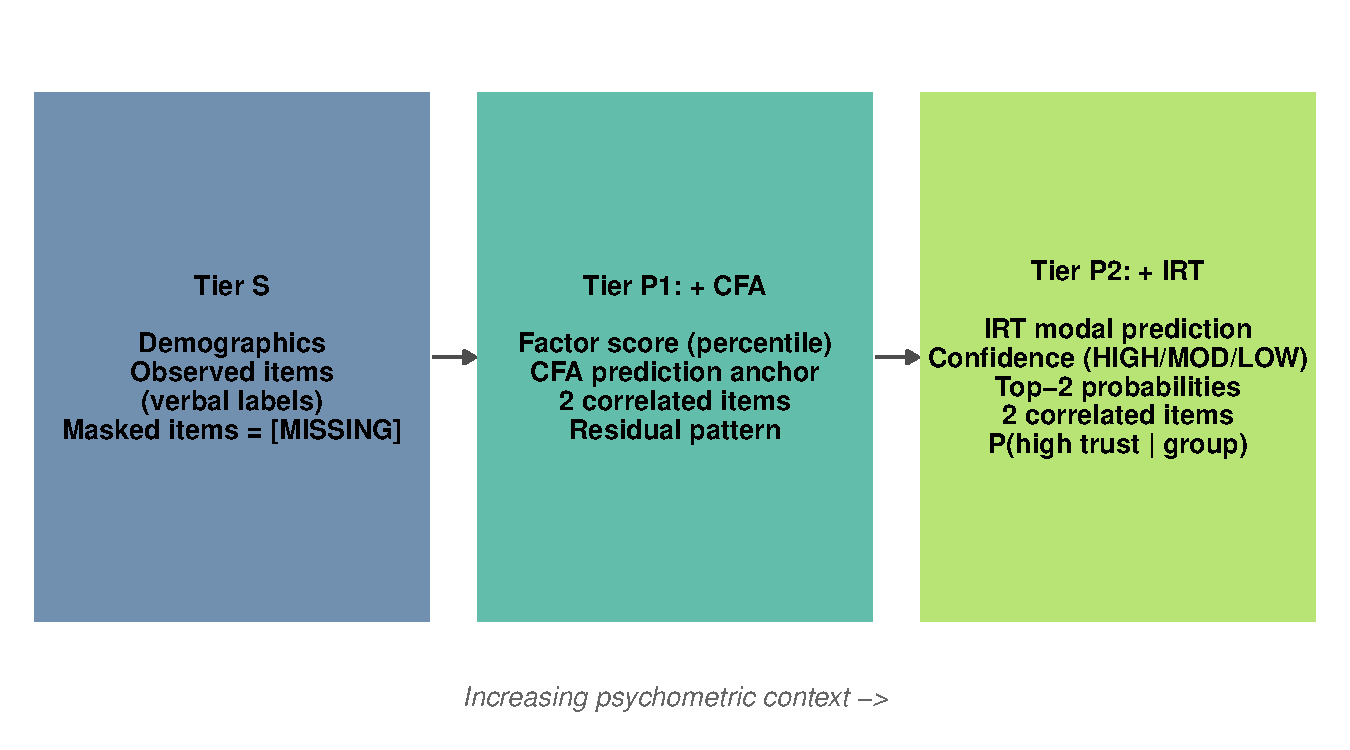
\includegraphics{final_paper_linares_files/figure-pdf/unnamed-chunk-2-1.pdf}

}

\end{figure}%

Three tiers are defined for LLMs in Figure 1, each adding progressively
richer psychometric context. Prompts communicate model conclusions
rather than raw parameters, early designs providing raw loadings,
discrimination values, and thresholds asked LLMs to predict from
scratch; consistently underperforming the IRT baseline. The production
design, which we call the model-then-adjust paradigm, provides the
model's conclusion as a starting point. For each masked item at P2, the
LLM receives the IRT modal category, a confidence label, the two most
correlated observed items with directional residual implications, and a
prescriptive adjustment signal. Five few-shot exemplars spanning the
latent spectrum (i.e., low/keep, moderate/adjust up, high/adjust down)
demonstrate when and how to adjust. The system prompt establishes a
psychometrician persona whose job is to refine predictions, not decide
whether to keep or change them. Note that traditional methods at P1/P2
also see the complete training response matrix, giving them an
information advantage over LLMs; the methodologically fair comparison is
therefore LLM tiers against traditional methods at S. Traditional
methods are evaluated at S only in the main analysis since this is the
most likely scenario of how imputations are carried out. Appendix B
presents the full prompting design.

\subsection{Imputation Models}\label{imputation-models}

We deploy Claude Sonnet 4.6 (i.e., Anthropic API, batch size 50) and
Llama 4 Maverick (i.e., OpenRouter, batch size 25) for imputation tasks
called via ellmer (\citeproc{ref-wickham2025}{Wickham, 2025}). Two
traditional benchmarks mixgb (\citeproc{ref-chen2016}{Chen \& Guestrin,
2016}) and miceRanger (\citeproc{ref-wright2017}{Wright \& Ziegler,
2017}) are used as comparisons. All methods use \(m = 5\) multiple
imputations with majority vote. For traditional methods, this follows
standard multiple imputation practice. For LLMs, five runs per condition
are generated at graduated temperatures (i.e., 0.01, 0.10, 0.20, 0.30,
0.40) to introduce controlled stochasticity, with the modal prediction
across runs as the final imputation.

\subsection{Out-of-Sample Evaluation
Design}\label{out-of-sample-evaluation-design}

We partition each survey dataset into five folds and for each fold
create a training/test split. The five-fold structure serves two
purposes. First, it prevents information leakage: psychometric models
(i.e., CFA and IRT) are fit to training data only, and the resulting
parameters feed into the LLM prompts. Without this separation, the
measurement model would have already seen the test respondents' item
responses, contaminating the out-of-sample evaluation. Second, the five
folds provide independent replications for variance estimation, which is
required for the Nadeau-Bengio corrected \(t\)-tests used for pairwise
method comparisons (\citeproc{ref-nadeau2003}{Nadeau \& Bengio, 2003}).
Note that cross-validation here does not serve its conventional purpose
of hyperparameter tuning, neither the LLMs nor the tree based methods
(i.e., which use default settings) have parameters selected via
cross-validation. Random masking of 1--4 items per test respondent is
shared across all methods and tiers. Three CFA/IRT model fits are
estimated per fold for RQ2 (i.e., ground truth, deletion, imputed), and
a fourth condition (i.e., mixgb S) is added for the RQ3 item parameter
comparison. These conditions are presented in Figure 2.

One aspect of the refit procedure warrants explicit clarification. The
\(m = 5\) imputations per cell collapse to a single modal prediction
(LLMs) or majority vote (tree-based methods) before entering the
test-fold response matrix, and the subsequent CFA and IRT refits treat
these imputed values as if they were observed. This is a
single-imputation treatment: we do not propagate within-imputation
variance across the refit via Rubin's rules. The choice is deliberate.
RQ2 and RQ3 evaluate point-estimate recovery of known ground-truth
parameters, so pooling standard errors across imputations would
complicate the Biemer decomposition without changing the \(\Delta a\),
response-variance, or \(\theta\) recovery quantities that answer the
research questions. Full Rubin's-rules pooling is a natural extension
for inferential applications and we flag it in Limitations.

\begin{figure}[H]

\caption{CFA/IRT Model Fit Conditions per Fold. Three measurement models
are estimated per fold for RQ2, with a fourth (mixgb S) added for the
RQ3 item-parameter comparison. Ground truth uses complete data; listwise
deletion excludes masked respondents; imputed retains the full sample
with predicted values replacing masked items, which enter the refit as
if observed.}

{\centering 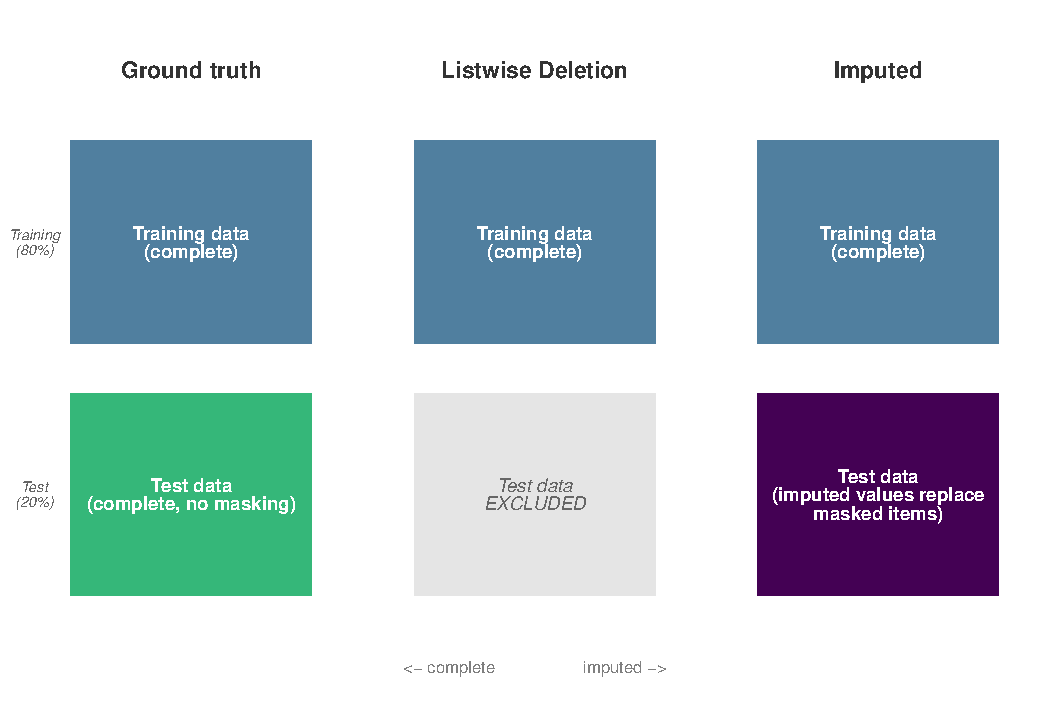
\includegraphics{final_paper_linares_files/figure-pdf/unnamed-chunk-3-1.pdf}

}

\end{figure}%

\subsection{Evaluation Metrics}\label{evaluation-metrics}

Each research question is evaluated with metrics targeting a specific
level of analysis and mapping onto the Biemer
(\citeproc{ref-biemer2010}{2010}) decomposition of total error into
systematic and variable components.

\emph{RQ1: Item-level measurement error.} The primary metric is
quadratic weighted kappa (\citeproc{ref-cohen1968}{Cohen, 1968}),
defined as

\[W\kappa = 1 - \frac{\sum_{i,j} w_{ij} \, O_{ij}}{\sum_{i,j} w_{ij} \, E_{ij}}\]

where \(O_{ij}\) and \(E_{ij}\) are observed and expected frequencies in
the \(K \times K\) confusion matrix, and quadratic weights
\(w_{ij} = (i - j)^2 / (K - 1)^2\) penalize predictions further from the
true category more heavily. The best-performing LLM-tier and traditional
method are carried forward to RQ2 and RQ3.

\emph{RQ2: Person-level measurement error.} For each method-tier
combination, we refit CFA and IRT on the combined training and imputed
test data (with imputed values treated as observed, as described above),
and compare the resulting latent variable estimates against the ground
truth. The Pearson correlation (\(r\)) between ground truth and imputed
captures rank preservation, whether respondents maintain their relative
positions after imputation. The regression slope captures scale fidelity
via

\[\theta_{\text{imputed}} = \beta_0 + \beta_1 \, \theta_{\text{gold}} + \varepsilon\]

where \(\beta_1 = 1.0\) indicates perfect scaling, values below 1.0
indicate centripetal compression\footnote{Centripetal compression is the
  tendency of predicted values to be pulled toward the center of the
  scale, overpredicting low responses and underpredicting high ones.},
and values above 1.0 indicate expansion.

\emph{RQ3: Instrument-level measurement error.} We assess what
imputation does to the measurement model itself by refitting the
psychometric models on four conditions per fold: ground truth (i.e.,
full data), listwise deletion (i.e., training only), best performing LLM
and traditional benchmark. Across experiment conditions, we extract item
parameters and compute the discrimination shift
\(\Delta a_{jk} = a_{jk}^{\text{imputed}} - a_{jk}^{\text{gold}}\) per
item \(j\) per fold \(k\). The Biemer (\citeproc{ref-biemer2010}{2010})
decomposition partitions the resulting MSE into

\[\text{MSE}_j = \underbrace{\left(\overline{\Delta a_j}\right)^2}_{\text{Bias}^2} + \underbrace{\overline{\left(\Delta a_j - \overline{\Delta a_j}\right)^2}}_{\text{Variance}}\]

where the \(\text{Bias}^2\) term captures systematic directional
distortion of item parameters and the Variance term captures random
fluctuation across folds; their ratio quantifies how much of the
measurement model distortion is systematic versus random. Item-level
response variance is also compared across conditions to assess whether
imputation shrinks the spread of responses.

\section{Results}\label{results}

\subsection{Item-Level Measurement
Error}\label{item-level-measurement-error}

The first research question asks whether communicating progressively
richer psychometric model information reduces item-level measurement
error, and how performance degrades as the proportion of masked items
within a scale increases. We evaluate Claude Sonnet and Maverick across
three information tiers alongside mixgb and miceRanger at the first
tier, using quadratic weighted kappa (\(W\kappa\)) as the primary metric
and exact-match accuracy as the secondary metric.

Claude Sonnet improves monotonically from S (\(W\kappa\) = .645) to P1
(.667) to P2 (.675) on the LAPOP 7-point scale, and from .550 to .559 to
.579 on the Latinobarómetro 4-point scale. Maverick shows a similar but
weaker upward trajectory on both surveys. At S---the fair
comparison---Claude Sonnet (\(W\kappa\) = .645 LAPOP, .550 LB)
outperforms mixgb (.615, .463) and miceRanger (.561, .504) on both
surveys.

Figure 3 extends this analysis by partitioning respondents into low
(1--2 items) and high (3--4 items) masking intensity. On LAPOP, all
methods are stable or improve slightly under heavier masking, reflecting
the 12-item scale's redundancy---enough observed items remain to anchor
predictions. On Latinobarómetro, where masking 3--4 of 6 items leaves
just 2--3 observed responses, the methods diverge sharply. Claude Sonnet
P2 declines modestly from .612 to .567, while mixgb S collapses from
.604 to .399---a 34\% degradation. This demonstrates that psychometric
context engineering provides the greatest value when the imputation task
is hardest: short scales with high item nonresponse. The psychometric
anchor sustains the LLM's predictions where tree-based methods, reliant
on the few remaining observed items, lose their signal. On the basis of
these results, Claude Sonnet at P2 is selected as the L2L representative
and mixgb at S as the traditional benchmark for subsequent analyses.

\begin{figure}[H]

\caption{LLM imputation is robust to masking intensity; traditional
methods collapse on shorter scales when more items are missing.}

{\centering 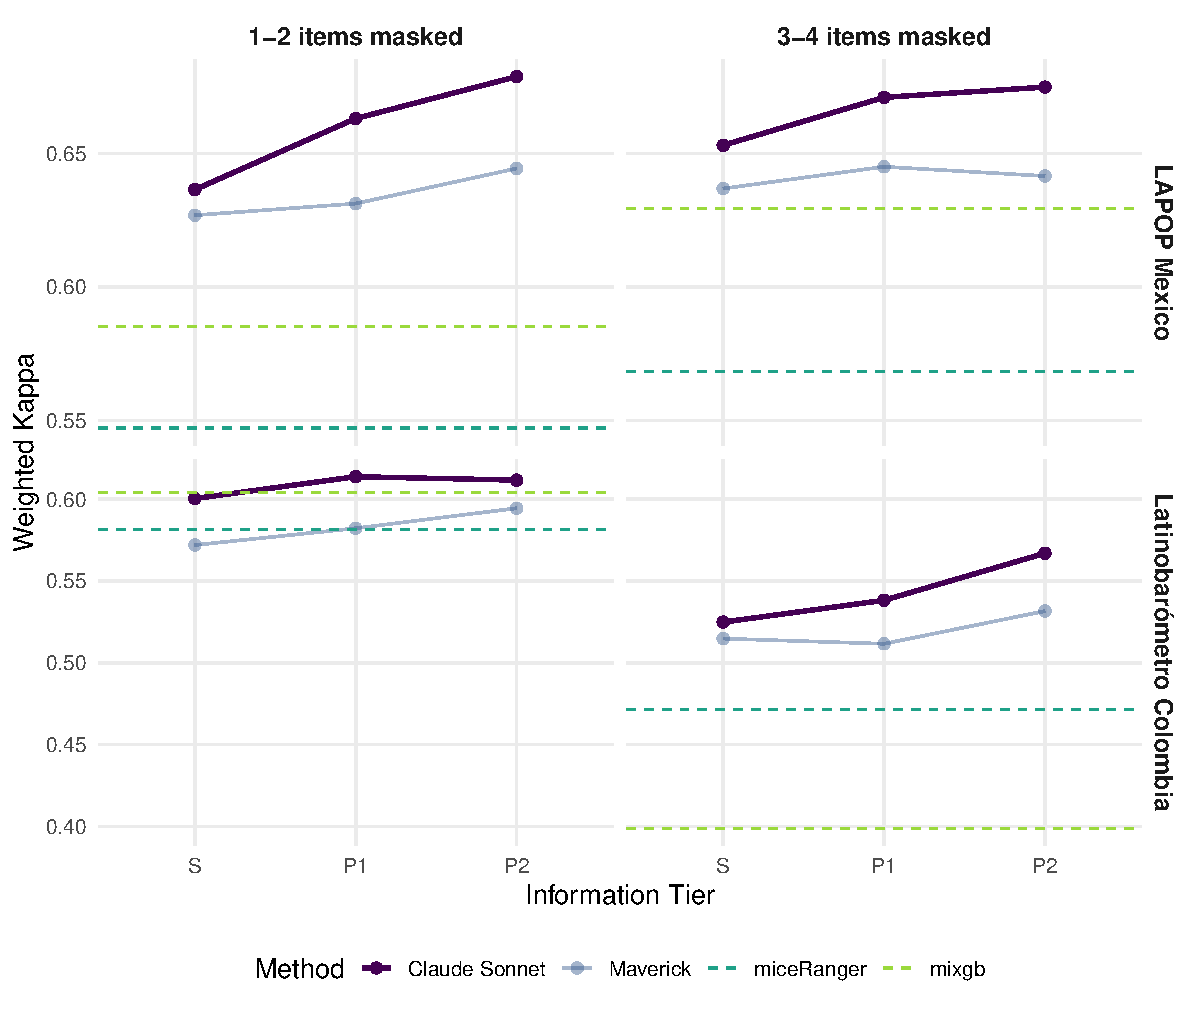
\includegraphics{final_paper_linares_files/figure-pdf/unnamed-chunk-4-1.pdf}

}

\end{figure}%

\subsection{Person-Level Measurement
Error}\label{person-level-measurement-error}

The second research question asks whether item-level improvements
translate to recovery of respondents' positions on the latent trust
construct. For each method-tier combination, CFA and IRT models are
refit on the combined training and imputed test data, and the resulting
IRT \(\theta\) estimates for test respondents are compared against the
ground truth. Rank preservation (\(r\)) and scale fidelity (regression
slope) capture two complementary dimensions of person-level measurement
error. Figure 4 plots \(\theta_{\text{gold}}\) against
\(\theta_{\text{imputed}}\) for Claude P2 and mixgb S across all folds,
with the regression fit (solid) and identity line (dashed) indicating
the degree of recovery.

\begin{figure}[H]

\caption{Claude P2 preserves latent score range on both surveys (slope
approx. 1.0); mixgb S compresses the Latinobarometro distribution by
11\%}

{\centering 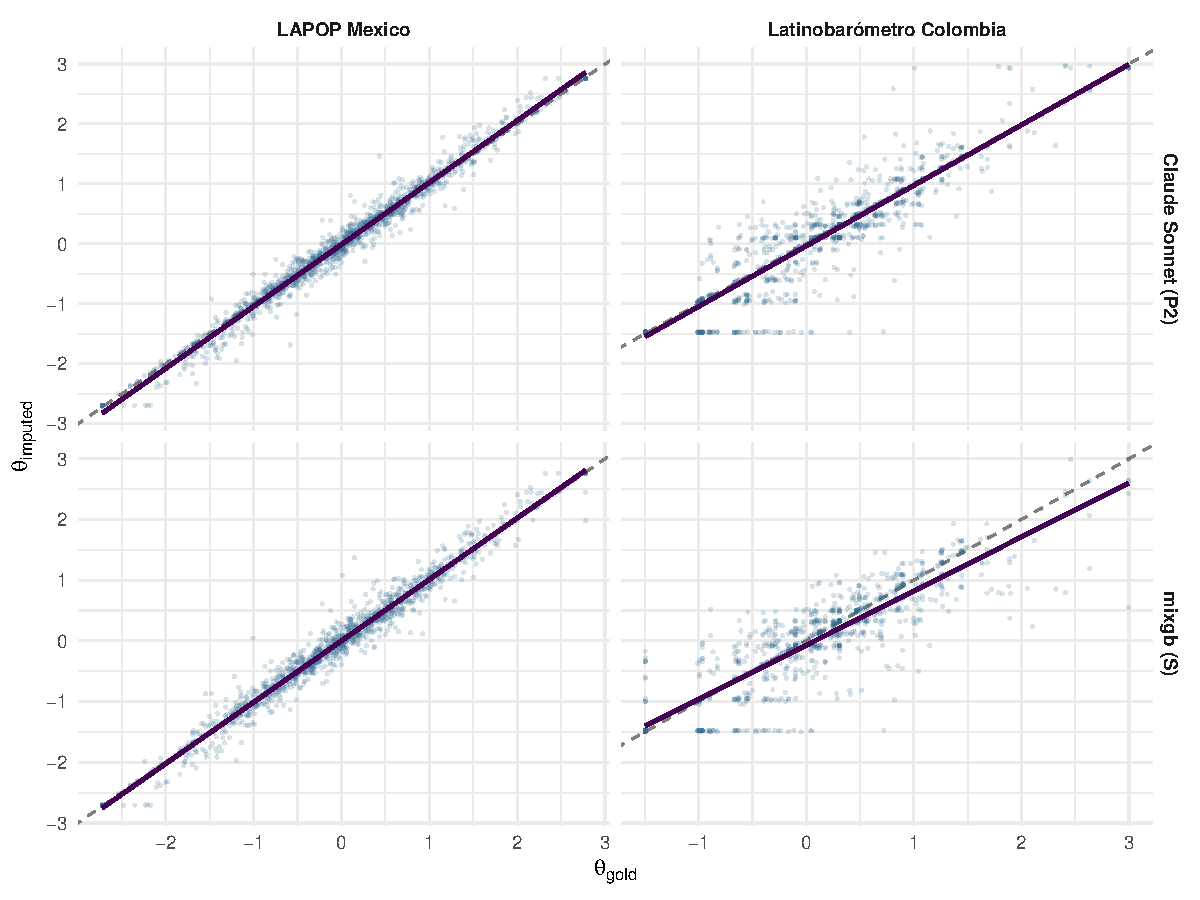
\includegraphics{final_paper_linares_files/figure-pdf/unnamed-chunk-5-1.pdf}

}

\end{figure}%

All methods preserve the rank ordering of respondents on the latent
construct with high fidelity. On the LAPOP 12-item scale, correlations
between ground truth and imputed \(\theta\) exceed \(r\) = .98 for every
method at every tier, with Claude Sonnet achieving \(r\) = .989 at S and
.988 at P2. The near-ceiling correlations indicate that all methods,
regardless of tier, correctly recover the rank ordering of high-trust
versus low-trust respondents on the 12-item scale. On the shorter
Latinobarómetro 6-item scale, correlations are lower but still strong:
Claude Sonnet ranges from \(r\) = .930 (S) to .924 (P2), outperforming
mixgb S (\(r\) = .895) by a meaningful margin. LLM-based imputation
preserves construct ordering more accurately than tree-based imputation
on both surveys.

The regression slope reveals where person-level measurement error
concentrates. Claude Sonnet at P2 produces slopes of 1.03 (LAPOP) and
1.01 (Latinobarómetro)---near-perfect scale fidelity with minimal
distortion of the \(\theta\) range. In contrast, mixgb at S shows slope
= 1.01 on LAPOP but 0.89 on Latinobarómetro, indicating 11\% centripetal
compression of the latent distribution on the shorter scale. This means
that while mixgb correctly orders respondents relative to one another,
it systematically underestimates the distance between high-trust and
low-trust individuals on the 4-point scale. Claude Sonnet at P2 avoids
this compression, maintaining both the ordering and the spread of the
latent construct.

\subsection{Instrument-Level Measurement
Error}\label{instrument-level-measurement-error}

The third research question asks what imputation does to the measurement
model itself. In the Graded Response Model, the discrimination parameter
(\(a_j\)) quantifies how sharply an item differentiates between
respondents at different levels of the latent trait. We refit IRT-GRM on
four conditions per fold (e.g., gold, deletion, Claude P2, mixgb S),
extract discrimination parameters, compute
\(\Delta a_j = a_j^{\text{imputed}} - a_j^{\text{gold}}\) per item per
fold, and decompose the resulting MSE into
\(\text{Bias}^2 + \text{Variance}\) following Biemer
(\citeproc{ref-biemer2010}{2010}).

Both imputation methods inflate item discrimination relative to the gold
standard (see Appendix C). Every item under both Claude P2 and mixgb S
shows positive \(\Delta a\). On LAPOP, mean \(\Delta a\) is \(+0.09\)
for Claude P2 and \(+0.05\) for mixgb S; on Latinobarómetro, \(+0.20\)
and \(+0.05\) respectively. This universal positive direction
demonstrates that discrimination inflation is an inherent consequence of
item imputation---any method that produces responses more consistent
with the latent factor than the original responses will tighten
inter-item covariance and inflate discrimination. The magnitudes are
small, less than 5\% relative distortion on LAPOP, but the composition
of the error differs. Claude P2's distortion is predominantly
systematic: 89\% of total MSE on LAPOP and 86\% on Latinobarómetro is
attributable to \(\text{Bias}^2\), while mixgb S shows a more balanced
profile (75\% and 33\%). Deletion introduces near-zero bias
(\(\Delta a \approx 0\)) but substantial variance from sample reduction.
These structurally distinct profiles mean that the imputation decision
is not which method introduces less total error, but which error
structure is more tolerable for the intended analysis (see Appendix D
for all method \(\times\) tier combinations).

Despite introducing more discrimination bias, Claude P2 preserves
item-level response variance better than mixgb S on the shorter
Latinobarómetro scale. On 5 of 6 LB items, mixgb S shrinks item variance
more than Claude P2 (i.e., Congress: \(-2.80\%\) vs.~\(-1.67\%\);
Judiciary: \(-2.57\%\) vs.~\(-1.50\%\)). On LAPOP, variance shrinkage is
comparable across both methods (mean \(\approx -0.5\%\)). This
decoupling means more discrimination bias but less variance shrinkage,
suggesting that the two methods introduce instrument-level measurement
error through different mechanisms.

Figure 5 decomposes the total discrimination MSE for each item into its
systematic (\(\text{Bias}^2\), solid) and random (Variance, faded)
components, with Claude P2 and mixgb S shown as paired bars for direct
comparison. Labels report total MSE followed by the percentage
attributable to \(\text{Bias}^2\) in parentheses. For example, ``0.026
(89\%)'' means total MSE is 0.026 and 89\% of that distortion is
systematic. Items are ordered by gold-standard discrimination, with the
highest-discriminating items at the top. Claude P2 shows consistently
higher MSE than mixgb S, but with a much larger systematic component
(85--98\% \(\text{Bias}^2\)), and mixgb S shows lower total MSE but with
more random error, particularly on Latinobarómetro where only 33\% of
MSE is systematic. The practical implication is that Claude P2's error
is predictable and potentially correctable through post-hoc adjustment,
while mixgb S's error is partly random and harder to address. Both
methods produce small absolute MSE values (i.e., all items below 0.10 on
LAPOP), reinforcing that the distortion is modest in applied terms
despite the structural differences.

\begin{figure}[H]

\caption{Claude P2 distortion is predominantly systematic (solid) while
mixgb S shows more random error (gap between solid and faded). Full bar
= total MSE; solid portion = Bias². Labels show total MSE and percent
systematic.}

{\centering 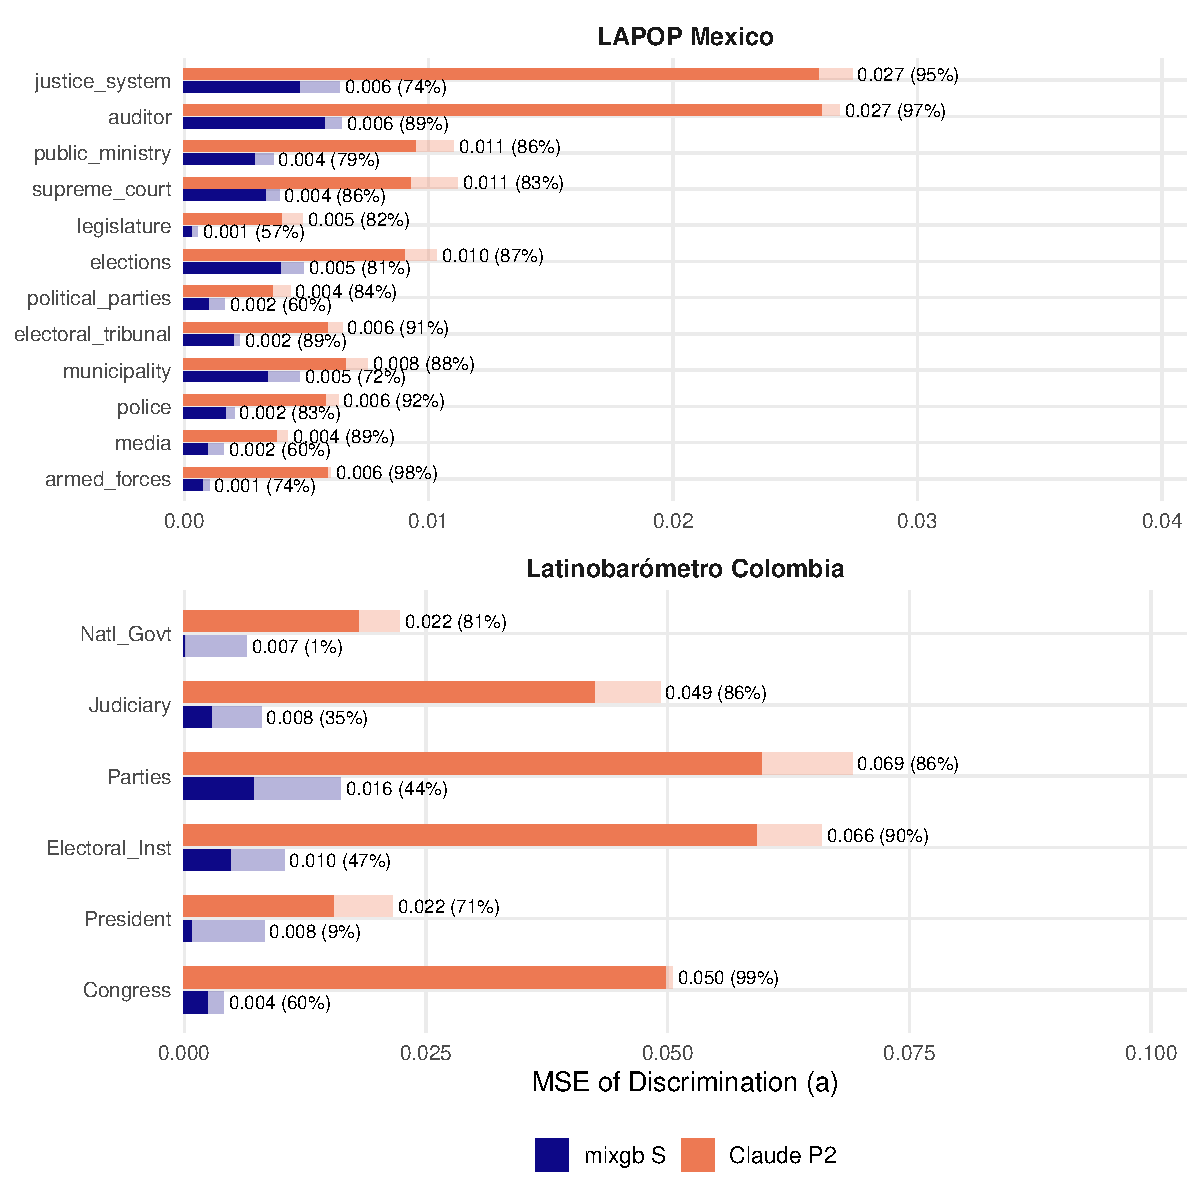
\includegraphics{final_paper_linares_files/figure-pdf/unnamed-chunk-6-1.pdf}

}

\end{figure}%

\section{Discussion}\label{discussion}

This study introduced the Latent-to-Language framework and evaluated it
within the Total Survey Error paradigm, asking whether translating
psychometric model conclusions into natural language prompts could
reduce measurement error introduced during item imputation, and whether
the resulting error could be decomposed and quantified at the item,
person, and instrument levels. To our knowledge, this is the first study
to leverage psychometric model conclusions as structured context for
LLM-based multi-item imputation, and the first to decompose the
resulting measurement error at three levels within the TSE framework.
Four findings merit discussion.

\subsection{Discrimination Inflation Is Universal, Not
Method-Specific}\label{discrimination-inflation-is-universal-not-method-specific}

Perhaps the most important finding is that discrimination inflation is
not unique to LLM-based imputation. Both approaches inflated
discrimination in the same direction on nearly every item. Any
researcher who imputes missing scale items and refits a measurement
model will obtain item parameters that overstate how sharply items
differentiate between respondents. Within the TSE framework
(\citeproc{ref-biemer2010}{Biemer, 2010}), this constitutes systematic
measurement error introduced at the imputation stage, one that is rarely
examined because few researchers compare post-imputation parameters
against a complete-data baseline.

Does the distortion matter? In absolute terms, the magnitudes are small
enough that substantive conclusions would not change. What differs is
the error composition. The LLM's error is predominantly systematic:
predictable, directional, and correctable through post-hoc adjustment.
The tree ensemble's error splits more evenly between systematic and
random components, making it harder to characterize after the fact. If
the priority is parameter stability across replications, the LLM's
predictable profile may be preferable despite higher total MSE. If the
priority is unbiasedness, the tree ensemble's lower systematic component
may be the better choice.

\subsection{Variance Preservation and Construct
Recovery}\label{variance-preservation-and-construct-recovery}

We did not anticipate that the method with more discrimination bias
would preserve item variance better. This decoupling suggests different
compression mechanisms: tree-based methods impute toward conditional
modes, uniformly tightening variance, while the LLM can deviate from the
mode when contextual signals point elsewhere, preserving response spread
even as covariance tightens.

For scale-level analyses like mean scores or group comparisons, either
mechanism is tolerable because construct ordering is preserved.
Item-level analyses such as DIF testing or adaptive item calibration are
more sensitive, and here the LLM's better variance preservation on short
scales offers a practical advantage. The construct recovery results
reinforce this: both methods maintain rank ordering, but the tree
ensemble compresses the latent distribution on the shorter scale,
pulling extremes toward the center. For researchers using short scales
in SMS surveys, web panels, or ecological momentary assessment, this
compression could attenuate treatment effects that depend on the tails
of the distribution.

\subsection{Prior-Attitude
Interference}\label{prior-attitude-interference}

LLMs carry semantic priors from their training corpus that can conflict
with population-specific attitudes, a source of error with no analog in
traditional imputation. When the LLM's world knowledge about an
institution diverges from the survey population's actual attitudes, the
imputed responses reflect the training distribution rather than the
respondent's true position. The bias is not random: it appears on the
same items, in the same direction, across folds.

The systematic bias also shows a clear item-level pattern on the longer
LAPOP scale. Appendix C Table C1 reports \(|\Delta a_j|\) alongside each
item's gold-standard discrimination, and the two quantities covary
closely: the highest-discrimination items (justice\_system at
\(a = 3.30\) and auditor at \(a = 2.97\)) carry the largest absolute
inflation (\(\Delta a \approx +0.16\) on each), roughly double what
appears on the lowest-discrimination items such as armed\_forces and
media (\(\Delta a\) between +0.06 and +0.08). The Latinobarómetro
pattern is less clean. Natl\_Govt has the scale's highest gold-standard
discrimination yet only middling inflation (\(\Delta a = +0.13\)), while
Parties, Electoral\_Inst, and Congress share similar mid-range
discrimination but show roughly double that inflation (\(\Delta a\)
between +0.22 and +0.24). Together these patterns suggest that
systematic bias emerges from an interaction between an item's factor
loading and the specificity of the LLM's training-corpus content for
that institution. Where the latent factor pulls hardest and the model
holds strong priors, the bias is largest.

LLM-based imputation therefore requires item-level diagnostics before
deployment. Signed error patterns by response category can identify
which items are affected, allowing researchers to exclude them or apply
corrections. This is especially important in cross-national research,
where the same institution may carry different connotations across
populations.

\subsection{Anchoring-Flexibility
Tradeoff}\label{anchoring-flexibility-tradeoff}

Over the course of developing the L2L prompt architecture, we
encountered an unexpected tension: the same information that improves
item-level accuracy can distort the measurement model by suppressing
independent reasoning. Early designs provided raw parameters like
loadings and thresholds, which produced worse predictions than the IRT
baseline alone. Replacing them with model conclusions (modal
predictions, confidence labels, adjustment directions) resolved this and
enabled the monotonic tier improvement. But when conclusions were too
precise, the LLM stopped reasoning. Given explicit probability
distributions, it simply rounded the IRT prediction to the nearest
integer.

The practical lesson: more psychometric detail does not always help. The
optimal prompt orients the LLM with a percentile or expected direction
without prescribing the outcome. We recommend starting with softer
anchors like CFA-level percentiles, escalating to IRT-level
probabilities only when item-level validation confirms the added
precision helps without compressing uniqueness. Shorter scales are more
susceptible to over-anchoring because concentrated probability
distributions leave less room for the LLM to deviate.

\subsection{Limitations}\label{limitations}

Several design choices constrain the generalizability of these findings.
First, items were masked under a MCAR mechanism (1--4 items per
respondent), which represents an optimistic scenario; real item
nonresponse patterns are more likely MAR or MNAR, and the performance of
both LLM and tree-based methods may degrade under informative
missingness. Second, maximum likelihood estimation treats ordinal
response categories as continuous, which is standard practice but
introduces approximation error in CFA and IRT model fits. Third, the IRT
specification is unidimensional; multidimensional constructs would
require richer psychometric context in the prompt architecture. Fourth,
evaluation is limited to two institutional trust scales in Latin
American populations (Mexico and Colombia), and generalizability to
other construct domains, cultures, and languages remains untested.
Fifth, survey weights were not incorporated, so all evaluation metrics
reflect case-level rather than population-level accuracy. Sixth, LLMs
carry semantic priors from their training corpus that can conflict with
population-specific attitudes. The armed forces item on the LAPOP scale
showed the largest negative signed error at high response categories,
indicating that when Mexican respondents report high trust in the armed
forces, the LLM systematically underpredicts. This pattern is consistent
with training-corpus coverage of Latin American militaries that runs
more negative than the institutional trust this population actually
reports. This prior-attitude interference constitutes a source of
systematic measurement error unique to LLM-based imputation, and
item-level signed error diagnostics should be considered a prerequisite
for any production deployment. Signed error by response category and
\(\Delta a\) by item currently serve as qualitative diagnostics;
converting these into quantitative deployment rules, for example
threshold-based flags on relative discrimination distortion, remains an
open research direction that we return to below.

Critically, this study framed L2L as a competitor to traditional
multiple imputation, comparing Claude Sonnet P2 against mixgb S in a
head-to-head design. The Biemer decomposition results suggest this
framing may be less productive than an enhancement framing. Claude P2
and mixgb S introduce complementary error structures, such that the LLM
contributes systematic discrimination inflation with preserved variance,
while the tree ensemble contributes more balanced error with greater
variance shrinkage. Rather than choosing between these methods, a more
promising approach may be to stack them: using the psychometric context
layer developed in L2L to augment, rather than replace, traditional
imputation workflows.

\subsection{Future Directions}\label{future-directions}

The complementary error structures identified in RQ3 motivate several
directions for future research. The most immediate is model stacking:
pooling multiple imputation datasets from tree-based methods and
allowing the LLM to serve as a governing reasoner that integrates
psychometric model conclusions with traditional imputation predictions
to produce a final imputation. Rubin's framework
(\citeproc{ref-rubin1986}{Rubin, 1986}) captures model uncertainty
through between-imputation variance, and combining structurally
different imputation engines would broaden this coverage. If the
systematic biases of the two methods partially offset in the pooled
ensemble, the combined approach could yield lower total measurement
model distortion than either method alone.

The anchoring-flexibility tradeoff identified in this study suggests
that prompt design for psychometric context engineering requires
calibration of anchoring strength, not simply maximization of
information density. Future work should systematically vary the
specificity of the psychometric anchor, for instance from no prediction
(tier S) through directional guidance (i.e., ``this respondent is above
average'') to point predictions with and without uncertainty
quantification, to map the anchoring-flexibility frontier for different
scale lengths and LLM architectures as they evolve with time.

The anchoring-flexibility finding emerged in part from a systematic
search over context-engineering parameters during framework development.
We varied batch composition (single respondent versus multi-respondent
batches), decoding temperature (0.01 to 0.40), output format (numeric
codes versus verbal category labels), and shot count (zero-shot versus
five-shot calibration), settling on the production configuration
reported in Methods. These variations shifted item-level weighted kappa
by small amounts in either direction, but none produced a configuration
with materially lower discrimination inflation at the instrument level.
This null result is informative. It suggests that systematic bias sits
upstream of the prompt itself, encoded in training-corpus priors that no
amount of context engineering can fully override. The tunable levers
shape item-level accuracy; the structural bias requires stacking with
methods that carry different priors, item-level routing, or
domain-adapted fine-tuning to address directly.

A more targeted variant is item-level routing, in which each masked item
is assigned to whichever method has lower historical MSE for that item's
discrimination parameter, leveraging the item-level Biemer decomposition
directly. This approach treats the L2L framework not as a standalone
imputation method but as one component within a broader imputation
architecture that allocates each prediction task to the method best
suited for it. Item-level routing further invites the development of
quantitative flagging rules. A diagnostic based on relative
discrimination distortion, such as \(|\Delta a_j| / a_j^{\text{gold}}\)
benchmarked against the deletion condition, could formalize the
currently qualitative deployment judgment and identify items where L2L
should be avoided or paired with a corrective adjustment before the
refit.

More broadly, the L2L framework should be tested under MAR and MNAR
missingness mechanisms, where the relationship between missingness and
the latent trait may interact with the psychometric anchoring in ways
not captured under MCAR. Extension to multidimensional constructs would
require richer prompt architectures capable of communicating
cross-factor dependencies. The prior attitude interference observed for
the armed forces item raises a broader concern for cross-national survey
research: the same institution may carry different connotations across
populations, meaning an imputation model validated in one country could
introduce systematic bias in another. Evaluation across other construct
domains, cultures, and languages is needed to determine how pervasive
this interference is and whether item-level signed error diagnostics can
reliably detect it before deployment. Finally, psychometric context
engineering may have applications beyond imputation, including adaptive
survey design where item selection is guided by real time latent trait
estimation, and automated quality monitoring where LLMs flag response
patterns inconsistent with the measurement model.

\newpage

\section{References}\label{references}

\phantomsection\label{refs}
\begin{CSLReferences}{1}{0}
\bibitem[\citeproctext]{ref-argyle2023}
Argyle, L. P., Busby, E. C., Fulda, N., Gubler, J. R., Rytting, C., \&
Wingate, D. (2023). Out of one, many: Using language models to simulate
human samples. \emph{Political Analysis}, \emph{31}(3), 1--15.
\url{https://doi.org/10.1017/pan.2023.2}

\bibitem[\citeproctext]{ref-barari2024}
Barari, S., \& Lerner, J. (2024). \emph{Large language models and survey
research: A recap}. AAPOR.
\url{https://aapor.org/newsletters/large-language-models-and-survey-research-a-recap/}

\bibitem[\citeproctext]{ref-biemer2010}
Biemer, P. P. (2010). Total survey error: Design, implementation, and
evaluation. \emph{Public Opinion Quarterly}, \emph{74}(5), 817--848.
\url{https://doi.org/10.1093/poq/nfq058}

\bibitem[\citeproctext]{ref-biemer2003}
Biemer, P. P., \& Lyberg, L. E. (2003). \emph{Introduction to survey
quality}. Wiley. \url{https://doi.org/10.1002/0471458740}

\bibitem[\citeproctext]{ref-bisbee2024}
Bisbee, J., Clinton, J. D., Dorff, C., Kenkel, B., \& Larson, J. M.
(2024). Synthetic replacements for human survey data? {The} perils of
large language models. \emph{Political Analysis}, \emph{32}(4),
401--416. \url{https://doi.org/10.1017/pan.2024.5}

\bibitem[\citeproctext]{ref-brick1996}
Brick, J. M., \& Kalton, G. (1996). Handling missing data in survey
research. \emph{Statistical Methods in Medical Research}, \emph{5}(3),
215--238. \url{https://doi.org/10.1177/096228029600500302}

\bibitem[\citeproctext]{ref-brown2015}
Brown, T. A. (2015). \emph{Confirmatory factor analysis for applied
research} (2nd ed.). Guilford Press.
\url{https://psycnet.apa.org/record/2015-10560-000}

\bibitem[\citeproctext]{ref-vanbuuren2011}
Buuren, S. van, \& Groothuis-Oudshoorn, K. (2011). {mice}: Multivariate
imputation by chained equations in {R}. \emph{Journal of Statistical
Software}, \emph{45}(3), 1--67.
\url{https://doi.org/10.18637/jss.v045.i03}

\bibitem[\citeproctext]{ref-chalmers2012}
Chalmers, R. P. (2012). {mirt}: A multidimensional item response theory
package for the {R} environment. \emph{Journal of Statistical Software},
\emph{48}(6), 1--29. \url{https://doi.org/10.18637/jss.v048.i06}

\bibitem[\citeproctext]{ref-chen2016}
Chen, T., \& Guestrin, C. (2016). {XGBoost}: A scalable tree boosting
system. \emph{Proceedings of the 22nd ACM SIGKDD International
Conference on Knowledge Discovery and Data Mining}, 785--794.
\url{https://doi.org/10.1145/2939672.2939785}

\bibitem[\citeproctext]{ref-cohen1968}
Cohen, J. (1968). Weighted kappa: Nominal scale agreement provision for
scaled disagreement or partial credit. \emph{Psychological Bulletin},
\emph{70}(4), 213--220. \url{https://doi.org/10.1037/h0026256}

\bibitem[\citeproctext]{ref-latinobarometro2023}
Corporación Latinobarómetro. (2023). \emph{{Latinobar{ó}metro} 2023}.
\url{https://www.latinobarometro.org/}

\bibitem[\citeproctext]{ref-deayala2009}
de Ayala, R. J. (2009). \emph{The theory and practice of item response
theory}. Guilford Press.

\bibitem[\citeproctext]{ref-flora2004}
Flora, D. B., \& Curran, P. J. (2004). An empirical evaluation of
alternative methods of estimation for confirmatory factor analysis with
ordinal data. \emph{Psychological Methods}, \emph{9}(4), 466--491.
\url{https://doi.org/10.1037/1082-989X.9.4.466}

\bibitem[\citeproctext]{ref-fornell1981}
Fornell, C., \& Larcker, D. F. (1981). Evaluating structural equation
models with unobservable variables and measurement error. \emph{Journal
of Marketing Research}, \emph{18}(1), 39--50.
\url{https://doi.org/10.1177/002224378101800104}

\bibitem[\citeproctext]{ref-groves2004}
Groves, R. M. (2004). \emph{Survey errors and survey costs}. Wiley.
\url{https://doi.org/10.1002/0471725277}

\bibitem[\citeproctext]{ref-groves2010}
Groves, R. M., \& Lyberg, L. (2010). Total survey error: Past, present,
and future. \emph{Public Opinion Quarterly}, \emph{74}(5), 849--879.
\url{https://doi.org/10.1093/poq/nfq065}

\bibitem[\citeproctext]{ref-vonderheyde2025}
Heyde, L. von der, Haensch, A.-C., \& Wenz, A. (2025). Vox populi, vox
{AI}? {Using} large language models to estimate {German} vote choice.
\emph{Social Science Computer Review}.
\url{https://doi.org/10.1177/08944393251337014}

\bibitem[\citeproctext]{ref-holgado2010}
Holgado-Tello, F. P., Chacón-Moscoso, S., Barbero-García, I., \&
Vila-Abad, E. (2010). Polychoric versus {Pearson} correlations in
exploratory and confirmatory factor analysis of ordinal variables.
\emph{Quality \& Quantity}, \emph{44}(1), 153--166.
\url{https://doi.org/10.1007/s11135-008-9190-y}

\bibitem[\citeproctext]{ref-holtdirk2024}
Holtdirk, T., Assenmacher, D., Bleier, A., \& Wagner, C. (2024).
Fine-tuning large language models to simulate {German} voting behaviour.
\emph{OSF Preprints}. \url{https://doi.org/10.31219/osf.io/udz28}

\bibitem[\citeproctext]{ref-horn1965}
Horn, J. L. (1965). A rationale and test for the number of factors in
factor analysis. \emph{Psychometrika}, \emph{30}(2), 179--185.
\url{https://doi.org/10.1007/BF02289447}

\bibitem[\citeproctext]{ref-hu1999}
Hu, L., \& Bentler, P. M. (1999). Cutoff criteria for fit indexes in
covariance structure analysis: Conventional criteria versus new
alternatives. \emph{Structural Equation Modeling: A Multidisciplinary
Journal}, \emph{6}(1), 1--55.
\url{https://doi.org/10.1080/10705519909540118}

\bibitem[\citeproctext]{ref-jansen2023}
Jansen, B. J., Jung, S.-G., \& Salminen, J. (2023). Employing large
language models in survey research. \emph{Natural Language Processing
Journal}, \emph{4}, 100020.
\url{https://doi.org/10.1016/j.nlp.2023.100020}

\bibitem[\citeproctext]{ref-kline2016}
Kline, R. B. (2016). \emph{Principles and practice of structural
equation modeling} (4th ed.). Guilford Press.
\url{https://psycnet.apa.org/record/2015-56948-000}

\bibitem[\citeproctext]{ref-kreuter2010}
Kreuter, F., Olson, K., Wagner, J., Yan, T., Ezzati-Rice, T. M.,
Casas-Cordero, C., Lemay, M., Peytchev, A., Groves, R. M., \&
Raghunathan, T. E. (2010). Using proxy measures and other correlates of
survey outcomes to adjust for non-response: Examples from multiple
surveys. \emph{Journal of the Royal Statistical Society: Series A
(Statistics in Society)}, \emph{173}(2), 389--407.
\url{https://doi.org/10.1111/j.1467-985X.2009.00621.x}

\bibitem[\citeproctext]{ref-lapop2023}
LAPOP Lab. (2023). \emph{{AmericasBarometer} 2023}. Vanderbilt
University. \url{https://www.vanderbilt.edu/lapop/}

\bibitem[\citeproctext]{ref-lerner2024}
Lerner, J. (2024). \emph{The promise \& pitfalls of {AI}-augmented
survey research}. NORC at the University of Chicago.
\url{https://www.norc.org/research/library/promise-pitfalls-ai-augmented-survey-research.html}

\bibitem[\citeproctext]{ref-little2002}
Little, R. J. A., \& Rubin, D. B. (2002). \emph{Statistical analysis
with missing data} (2nd ed.). Wiley.
\url{https://doi.org/10.1002/9781119013563}

\bibitem[\citeproctext]{ref-little2005}
Little, R. J., \& Vartivarian, S. L. (2005). Does weighting for
nonresponse increase the variance of survey means? \emph{Survey
Methodology}, \emph{31}(2), 161--168.
\url{https://www150.statcan.gc.ca/n1/pub/12-001-x/2005002/article/9044-eng.pdf}

\bibitem[\citeproctext]{ref-minaee2024}
Minaee, S., Mikolov, T., Nikzad, N., Chenaghlu, M., Socher, R.,
Amatriain, X., \& Gao, J. (2024). Large language models: A survey.
\emph{arXiv}. \url{https://arxiv.org/abs/2402.06196}

\bibitem[\citeproctext]{ref-nadeau2003}
Nadeau, C., \& Bengio, Y. (2003). Inference for the generalization
error. \emph{Machine Learning}, \emph{52}(3), 239--281.
\url{https://doi.org/10.1023/A:1024068626366}

\bibitem[\citeproctext]{ref-raykov2001}
Raykov, T. (2001). Estimation of congeneric scale reliability using
covariance structure analysis with nonlinear constraints. \emph{British
Journal of Mathematical and Statistical Psychology}, \emph{54}(2),
315--323. \url{https://doi.org/10.1348/000711001159582}

\bibitem[\citeproctext]{ref-rosseel2012}
Rosseel, Y. (2012). {lavaan}: An {R} package for structural equation
modeling. \emph{Journal of Statistical Software}, \emph{48}(2), 1--36.
\url{https://doi.org/10.18637/jss.v048.i02}

\bibitem[\citeproctext]{ref-rubin1986}
Rubin, D. B. (1986). Basic ideas of multiple imputation for nonresponse.
\emph{Survey Methodology}, \emph{12}(1), 37--47.
\url{https://www150.statcan.gc.ca/n1/en/pub/12-001-x/1986001/article/14439-eng.pdf?st=DuvW3mPc}

\bibitem[\citeproctext]{ref-samejima1969}
Samejima, F. (1969). Estimation of latent ability using a response
pattern of graded scores. \emph{Psychometrika Monograph Supplement},
\emph{34}(4, Pt. 2), 1--97. \url{https://doi.org/10.1007/BF03372160}

\bibitem[\citeproctext]{ref-vaswani2017}
Vaswani, A., Shazeer, N., Parmar, N., Uszkoreit, J., Jones, L., Gomez,
A. N., Kaiser, Ł., \& Polosukhin, I. (2017). Attention is all you need.
\emph{Advances in Neural Information Processing Systems}, \emph{30}.
\url{https://arxiv.org/abs/1706.03762}

\bibitem[\citeproctext]{ref-west2016}
West, B. T., Sakshaug, J. W., \& Aurelien, G. A. S. (2016). How big of a
problem is analytic error in secondary analyses of survey data?
\emph{PLoS ONE}, \emph{11}(6), e0158120.
\url{https://doi.org/10.1371/journal.pone.0158120}

\bibitem[\citeproctext]{ref-wickham2025}
Wickham, H. (2025). \emph{{ellmer}: Chat with large language models from
{R}}. \url{https://ellmer.tidyverse.org/}

\bibitem[\citeproctext]{ref-wright2017}
Wright, M. N., \& Ziegler, A. (2017). {ranger}: A fast implementation of
random forests for high dimensional data in {C++} and {R}. \emph{Journal
of Statistical Software}, \emph{77}(1), 1--17.
\url{https://doi.org/10.18637/jss.v077.i01}

\bibitem[\citeproctext]{ref-yen1984}
Yen, W. M. (1984). Effects of local item dependence on the fit and
equating performance of the three-parameter logistic model.
\emph{Applied Psychological Measurement}, \emph{8}(2), 125--145.
\url{https://doi.org/10.1177/014662168400800201}

\end{CSLReferences}

\appendix

\section{Psychometric Model Details}\label{apx-psychometrics}

\begin{table}
\caption{CFA Fit Statistics (Averaged Across 5 Training Folds)}\tabularnewline

\centering\begingroup\fontsize{10}{12}\selectfont

\begin{tabular}{lrrrrr}
\toprule
Survey & CFI & TLI & RMSEA & SRMR & omega\\
\midrule
LAPOP Mexico (12 items) & 0.957 & 0.945 & 0.076 & 0.030 & 0.921\\
Latinobarómetro Colombia (6 items) & 0.984 & 0.969 & 0.069 & 0.023 & 0.783\\
\bottomrule
\end{tabular}
\endgroup{}
\end{table}

\begin{figure}

\caption{\label{fig-apx-cfa-path}CFA Path Diagram for LAPOP Mexico Trust
Scale (Fold 1 Training). Standardized loadings on paths; freed residual
covariances between public ministry and auditor.}

\centering{

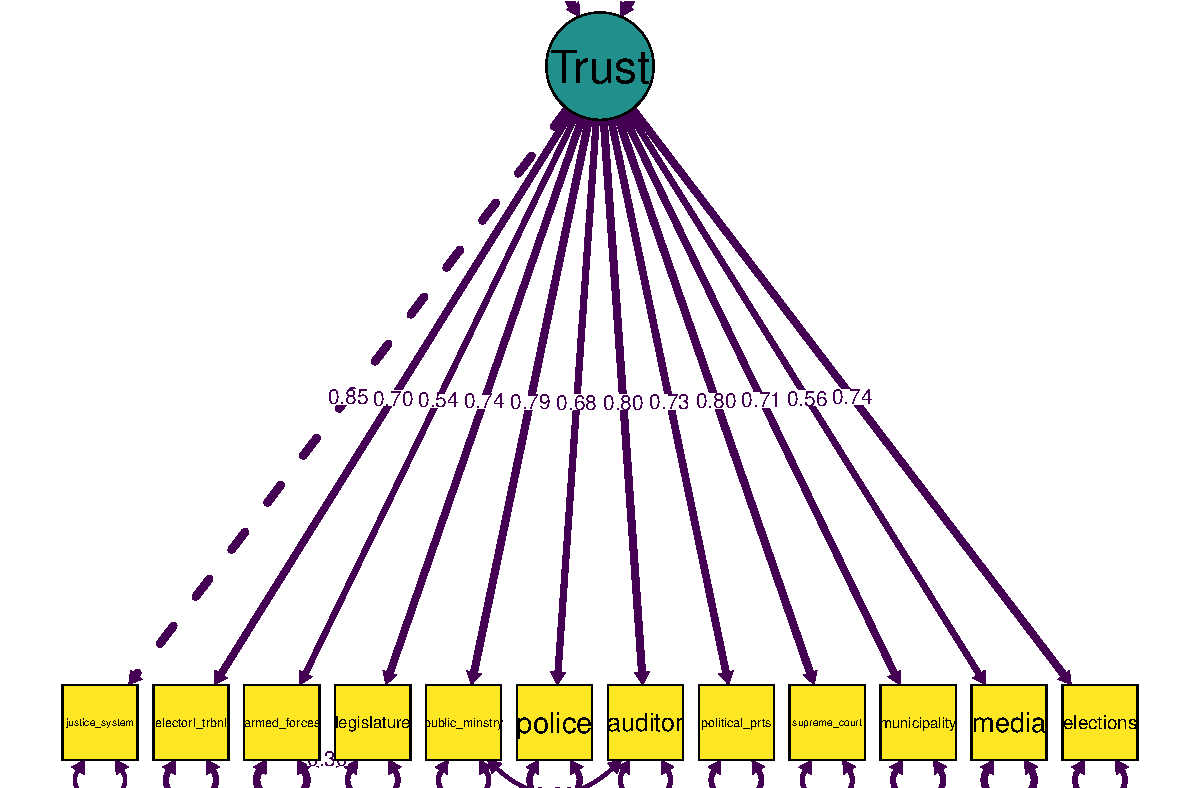
\includegraphics{final_paper_linares_files/figure-pdf/fig-apx-cfa-path-1.pdf}

}

\end{figure}%

\begin{figure}

\caption{\label{fig-apx-icc-lapop}IRT Category Probability Curves ---
LAPOP Mexico (Fold 1). Each panel shows one item; curves represent the
probability of each response category as a function of latent trust
(\(\theta\)). Higher discrimination items (e.g., justice\_system,
public\_ministry) show steeper, more separated curves.}

\centering{

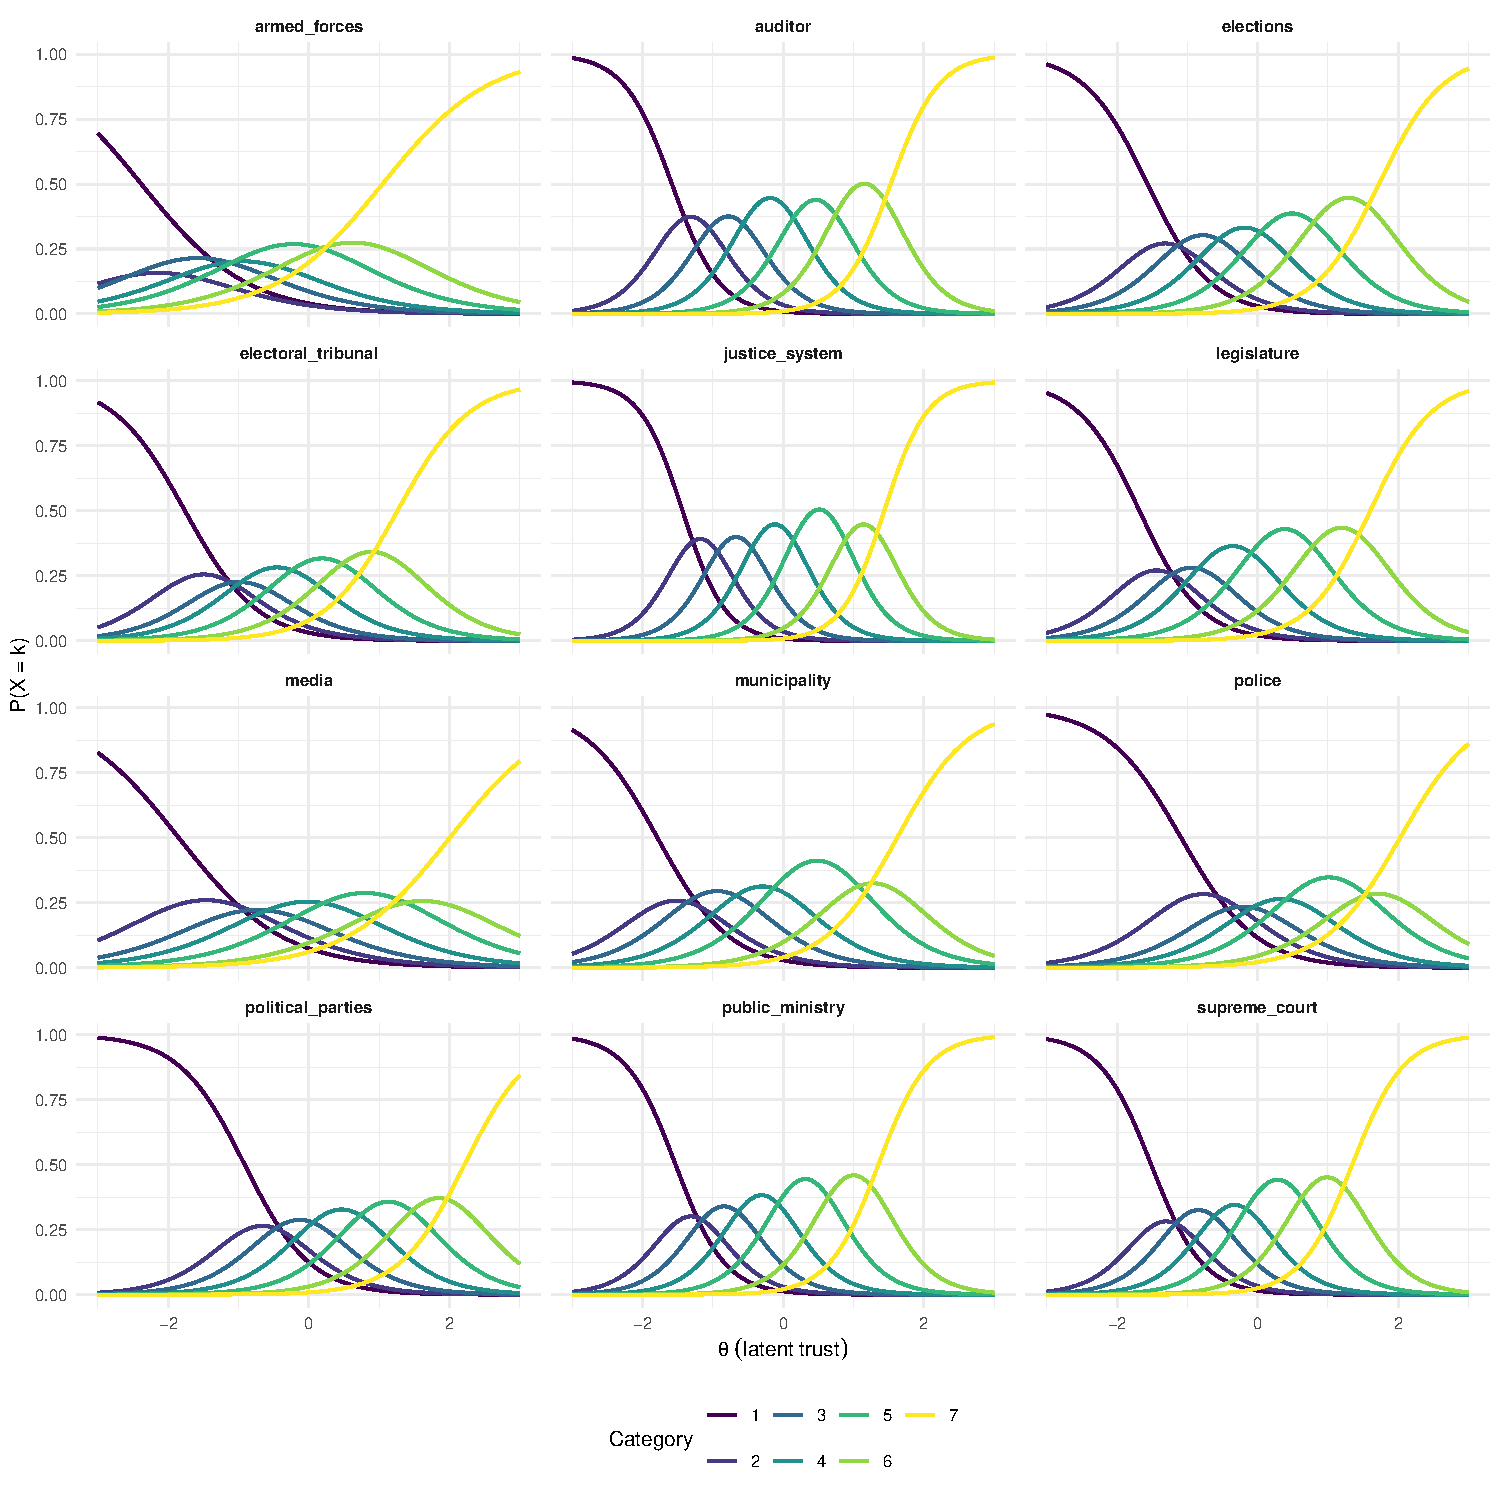
\includegraphics{final_paper_linares_files/figure-pdf/fig-apx-icc-lapop-1.pdf}

}

\end{figure}%

\section{Prompt Design}\label{apx-prompts}

Production prompts batch 25 respondents per API call (50 for Claude
Sonnet). For P1 and P2 tiers, three few-shot calibration examples from
training data are prepended to demonstrate when to keep versus adjust
the model prediction. The system prompt is identical across all tiers;
only the user prompt content changes.

\subsubsection{System Prompt (All Tiers)}\label{system-prompt-all-tiers}

\begin{verbatim}
You are a survey psychometrician with a PhD from the Joint Program
in Survey Methodology (JPSM) at the University of Maryland,
specializing in survey data science. You are reviewing an
institutional trust scale from a nationally representative survey
conducted in Mexico in 2023 where some item responses are missing
and need to be imputed.

Scale: 1 = no trust at all, 7 = a lot of trust

Your task: For each respondent, a statistical model provides a
starting-point prediction for each missing item. Your job is to
REFINE these predictions using information the model cannot
capture. The model only sees numerical patterns -- you can see
response consistency, demographic context, and institutional
meaning.

HOW TO REASON:
1. Start from the model prediction, then look at the RESIDUAL
   PATTERN. If this respondent consistently rates ABOVE or BELOW
   the model on observed items, the missing items almost certainly
   follow the same direction. Adjust accordingly -- this is the
   strongest signal.
2. Check the CORRELATED ITEMS. If the two most related observed
   items are both above (or below) the model, that is direct
   evidence to adjust in the same direction.
3. Consider DEMOGRAPHIC CONTEXT as a sanity check. If the model
   predicts a value that is unusual for this respondent's
   demographic group, that may warrant a small adjustment -- but
   respondent-level patterns always outweigh group averages.
4. Use DOMAIN KNOWLEDGE. Trust in armed forces is substantively
   different from trust in the judiciary. Consider what you know
   about how these specific institutions are perceived in this
   country.
5. When model confidence is LOW (the top category has <30%
   probability), the model is genuinely uncertain -- your
   contextual reasoning adds the most value here. Do not simply
   repeat the model prediction.
6. Trust scales exhibit HALO EFFECTS. If a respondent rates all
   observed institutions consistently high or low, the missing
   items almost certainly follow suit.
7. Your prediction must be an INTEGER on the scale
   (1 = no trust at all, 7 = a lot of trust).

OUTPUT: One line per respondent. Format:
row_id: item1=value, item2=value
No explanation. Only prediction lines.
\end{verbatim}

\subsubsection{Tier S User Prompt (No
Model)}\label{tier-s-user-prompt-no-model}

\begin{verbatim}
RESPONDENT 42:
  Demographics: Male | 30-44 | Secondary | Urban
  Observed trust ratings:
    justice_system = 5 (Moderate trust)
    electoral_tribunal = 4 (Some trust)
    public_ministry = 3 (Little trust)
    police = 6 (High trust)
    auditor = 4 (Some trust)
    political_parties = 2 (Very little trust)
    supreme_court = 5 (Moderate trust)
    municipality = 4 (Some trust)
    media = 3 (Little trust)
    elections = 5 (Moderate trust)
  Predict:
    armed_forces: [MISSING]
    legislature: [MISSING]
\end{verbatim}

\subsubsection{Tier P2 User Prompt (IRT
Augmented)}\label{tier-p2-user-prompt-irt-augmented}

\begin{verbatim}
RESPONDENT 42:
  Demographics: Male | 30-44 | Secondary | Urban
  Observed trust ratings:
    justice_system = 5 (Moderate trust)
    electoral_tribunal = 4 (Some trust)
    public_ministry = 3 (Little trust)
    police = 6 (High trust)
    auditor = 4 (Some trust)
    political_parties = 2 (Very little trust)
    supreme_court = 5 (Moderate trust)
    municipality = 4 (Some trust)
    media = 3 (Little trust)
    elections = 5 (Moderate trust)
  Overall pattern: This respondent consistently rates ABOVE
    the model (+0.5 avg) -> adjust predictions UPWARD
  MISSING ITEMS -- predict each:
    armed_forces: [MISSING]
      Model prediction: 4
      Confidence: MODERATE (4 at 35%, 5 at 20%)
        -- use residual pattern to refine
      Most informative observed items:
        police = 6 (model expected 5.2, +0.8 above
          -> suggests this item should also be ABOVE model)
        supreme_court = 5 (model expected 4.7, +0.3 above
          -> suggests this item should also be ABOVE model)
      Demographic context: For your group, P(high trust
        on armed_forces) = 48% vs. population 43%
    legislature: [MISSING]
      Model prediction: 4
      Confidence: MODERATE (4 at 33%, 5 at 25%)
        -- use residual pattern to refine
      Most informative observed items:
        justice_system = 5 (model expected 4.6, +0.4 above
          -> suggests this item should also be ABOVE model)
        electoral_tribunal = 4 (model expected 3.9, +0.1 above
          -- consistent with model)
      Demographic context: For your group, P(high trust
        on legislature) = 39% vs. population 35%
\end{verbatim}

\subsubsection{Few-Shot Calibration Examples (P1 and P2
Only)}\label{few-shot-calibration-examples-p1-and-p2-only}

Three training-fold exemplars spanning the latent spectrum are prepended
to the user prompt. Each shows the correct answer so the LLM learns when
to keep versus adjust.

\begin{verbatim}
CALIBRATION EXAMPLES (from training data):
These show when to keep the model vs. when to adjust.

Example (KEEP -- model confidence is high and respondent
  pattern is consistent):
  Demographics: Female | 45-59 | Higher education | Urban
  Observed: [observed items with verbal labels]
  Overall pattern: This respondent is close to model
    expectations (+0.1 avg) -> model predictions are
    likely accurate
  Predict:
    supreme_court: [MISSING]
      Model prediction: 4
      Confidence: MODERATE (4 at 38%)
      Most informative observed items:
        justice_system = 4 (model expected 4.1, -0.1 below
          -- consistent with model)
      -> Correct answer: 4
    media: [MISSING]
      Model prediction: 3
      Confidence: MODERATE (3 at 31%)
      Most informative observed items:
        political_parties = 3 (model expected 2.8, +0.2 above
          -- consistent with model)
      -> Correct answer: 3
  Output: 108: supreme_court=4, media=3

Example (ADJUST UP -- respondent consistently rates above
  model, uncertainty is high):
  Demographics: Male | 18-29 | Secondary | Rural
  Observed: [observed items with verbal labels]
  Overall pattern: This respondent consistently rates ABOVE
    the model (+1.2 avg) -> adjust predictions UPWARD
  Predict:
    police: [MISSING]
      Model prediction: 4
      Confidence: LOW (4 at 29%)
      Most informative observed items:
        municipality = 6 (model expected 4.8, +1.2 above
          -> suggests this item should also be ABOVE model)
      -> Correct answer: 5
  Output: 215: police=5

Example (ADJUST DOWN -- despite high trust overall, this
  item's pattern suggests lower):
  Demographics: Female | 60+ | Primary | Urban
  Observed: [observed items with verbal labels]
  Overall pattern: This respondent consistently rates BELOW
    the model (-0.9 avg) -> adjust predictions DOWNWARD
  Predict:
    armed_forces: [MISSING]
      Model prediction: 4
      Confidence: MODERATE (4 at 33%)
      Most informative observed items:
        elections = 3 (model expected 4.1, -1.1 below
          -> suggests this item should also be BELOW model)
      -> Correct answer: 3
  Output: 347: armed_forces=3

Now predict for the test respondents below.
\end{verbatim}

\section{IRT Discrimination Biemer
Decomposition}\label{apx-discrim-biemer}

This appendix presents the item-level and aggregate Biemer
(\citeproc{ref-biemer2010}{2010}) decomposition of IRT discrimination
parameter error (\(\Delta a\) = condition \(-\) gold) for Claude P2,
mixgb S, and listwise deletion.

\begin{table}
\caption{Item-Level Biemer Decomposition of IRT Discrimination --- Claude P2 and
mixgb S vs Gold Standard. Bias = mean \(\Delta a\) across 5 folds. MSE =
Bias\(^2\) + Variance.}\tabularnewline

\centering\begingroup\fontsize{9}{11}\selectfont

\resizebox{\ifdim\width>\linewidth\linewidth\else\width\fi}{!}{
\begin{tabular}{llrllrllr}
\toprule
Survey & Item & Gold a & Claude Bias & Claude MSE & Claude \%Sys & mixgb Bias & mixgb MSE & mixgb \%Sys\\
\midrule
LAPOP Mexico & justice\_system & 3.304 & +0.1611 & 0.0273 & 95.0 & +0.0689 & 0.0064 & 74.3\\
LAPOP Mexico & auditor & 2.968 & +0.1614 & 0.0268 & 97.2 & +0.0758 & 0.0065 & 89.1\\
LAPOP Mexico & public\_ministry & 2.792 & +0.0973 & 0.0110 & 85.7 & +0.0537 & 0.0037 & 79.1\\
LAPOP Mexico & supreme\_court & 2.548 & +0.0962 & 0.0112 & 82.8 & +0.0578 & 0.0039 & 85.9\\
LAPOP Mexico & legislature & 2.263 & +0.0632 & 0.0049 & 82.1 & +0.0180 & 0.0006 & 57.2\\
\addlinespace
LAPOP Mexico & elections & 2.209 & +0.0949 & 0.0103 & 87.0 & +0.0630 & 0.0049 & 80.9\\
LAPOP Mexico & political\_parties & 2.133 & +0.0603 & 0.0044 & 83.7 & +0.0316 & 0.0017 & 60.1\\
LAPOP Mexico & electoral\_tribunal & 1.994 & +0.0766 & 0.0065 & 90.6 & +0.0450 & 0.0023 & 89.0\\
LAPOP Mexico & municipality & 1.984 & +0.0812 & 0.0075 & 87.8 & +0.0584 & 0.0047 & 72.3\\
LAPOP Mexico & police & 1.918 & +0.0760 & 0.0063 & 91.7 & +0.0413 & 0.0021 & 83.1\\
\addlinespace
LAPOP Mexico & media & 1.367 & +0.0615 & 0.0043 & 88.8 & +0.0312 & 0.0016 & 59.9\\
LAPOP Mexico & armed\_forces & 1.333 & +0.0767 & 0.0060 & 98.0 & +0.0275 & 0.0010 & 73.5\\
Latinobarómetro Colombia & Natl\_Govt & 2.662 & +0.1343 & 0.0223 & 80.7 & -0.0071 & 0.0065 & 0.8\\
Latinobarómetro Colombia & Judiciary & 2.135 & +0.2061 & 0.0492 & 86.3 & +0.0531 & 0.0080 & 35.2\\
Latinobarómetro Colombia & Parties & 2.121 & +0.2443 & 0.0691 & 86.4 & +0.0846 & 0.0162 & 44.1\\
\addlinespace
Latinobarómetro Colombia & Electoral\_Inst & 2.035 & +0.2433 & 0.0660 & 89.7 & +0.0696 & 0.0104 & 46.7\\
Latinobarómetro Colombia & President & 2.005 & +0.1242 & 0.0216 & 71.4 & +0.0278 & 0.0083 & 9.3\\
Latinobarómetro Colombia & Congress & 1.993 & +0.2232 & 0.0505 & 98.7 & +0.0495 & 0.0041 & 59.8\\
\bottomrule
\end{tabular}}
\endgroup{}
\end{table}

\begin{table}
\caption{Aggregate Discrimination MSE --- Claude P2, mixgb S, and Deletion. Mean
across items per survey.}\tabularnewline

\centering\begingroup\fontsize{10}{12}\selectfont

\begin{tabular}{llrrrrr}
\toprule
Survey & Condition & Bias & Bias Sq. & Variance & MSE & \% Syst\\
\midrule
LAPOP Mexico & Claude P2 & 0.0922 & 0.009610 & 0.000933 & 0.010543 & 89.2\\
LAPOP Mexico & mixgb S & 0.0477 & 0.002574 & 0.000694 & 0.003268 & 75.4\\
LAPOP Mexico & Deletion & 0.0007 & 0.000001 & 0.003390 & 0.003392 & 0.0\\
Latinobarómetro Colombia & Claude P2 & 0.1959 & 0.040773 & 0.005682 & 0.046455 & 85.5\\
Latinobarómetro Colombia & mixgb S & 0.0462 & 0.003017 & 0.005910 & 0.008927 & 32.6\\
\addlinespace
Latinobarómetro Colombia & Deletion & 0.0034 & 0.000014 & 0.012179 & 0.012193 & 0.1\\
\bottomrule
\end{tabular}
\endgroup{}
\end{table}

\section{Full MSE Decomposition}\label{apx-mse-full}

This appendix presents the full Biemer (\citeproc{ref-biemer2010}{2010})
decomposition of item level mean squared error for all method \(\times\)
tier combinations.

\begin{table}
\caption{Biemer Decomposition of item level MSE: All Methods and Tiers}\tabularnewline

\centering\begingroup\fontsize{8}{10}\selectfont

\resizebox{\ifdim\width>\linewidth\linewidth\else\width\fi}{!}{
\begin{tabular}{lllccccc}
\toprule
Survey & Type & Method & Tier & Bias Sq. & Variance & MSE & \% Syst.\\
\midrule
LAPOP Mexico & Traditional & miceRanger & S & 0.0716 & 2.9258 & 2.9876 & 2.4\\
LAPOP Mexico & Traditional & mixgb & S & 0.0093 & 2.5277 & 2.5285 & 0.4\\
LAPOP Mexico & LLM & Maverick & S & 0.1070 & 2.1798 & 2.2795 & 4.7\\
LAPOP Mexico & LLM & Claude Sonnet & S & 0.0747 & 1.8672 & 1.9349 & 3.9\\
LAPOP Mexico & Traditional & miceRanger & P1 & 0.0775 & 2.6619 & 2.7305 & 2.8\\
LAPOP Mexico & Traditional & mixgb & P1 & 0.0078 & 2.3132 & 2.3132 & 0.3\\
LAPOP Mexico & LLM & Maverick & P1 & 0.0480 & 2.3069 & 2.3472 & 2.0\\
LAPOP Mexico & LLM & Claude Sonnet & P1 & 0.0385 & 1.9188 & 1.9509 & 2.0\\
LAPOP Mexico & Traditional & miceRanger & P2 & 0.1016 & 2.6569 & 2.7497 & 3.7\\
LAPOP Mexico & Traditional & mixgb & P2 & 0.0105 & 2.2057 & 2.2089 & 0.5\\
LAPOP Mexico & LLM & Maverick & P2 & 0.0192 & 2.3752 & 2.3865 & 0.8\\
LAPOP Mexico & LLM & Claude Sonnet & P2 & 0.0131 & 2.0515 & 2.0577 & 0.6\\
Latinobarómetro Colombia & Traditional & miceRanger & S & 0.0023 & 0.7225 & 0.7232 & 0.3\\
Latinobarómetro Colombia & Traditional & mixgb & S & 0.0206 & 0.6828 & 0.7019 & 2.9\\
Latinobarómetro Colombia & LLM & Maverick & S & 0.0370 & 0.5694 & 0.6051 & 6.1\\
Latinobarómetro Colombia & LLM & Claude Sonnet & S & 0.0182 & 0.5680 & 0.5847 & 3.1\\
Latinobarómetro Colombia & Traditional & miceRanger & P1 & 0.0075 & 0.6928 & 0.6987 & 1.1\\
Latinobarómetro Colombia & Traditional & mixgb & P1 & 0.0011 & 0.6522 & 0.6518 & 0.2\\
Latinobarómetro Colombia & LLM & Maverick & P1 & 0.0283 & 0.6936 & 0.7204 & 3.9\\
Latinobarómetro Colombia & LLM & Claude Sonnet & P1 & 0.0082 & 0.5754 & 0.5823 & 1.4\\
Latinobarómetro Colombia & Traditional & miceRanger & P2 & 0.0009 & 0.6813 & 0.6807 & 0.1\\
Latinobarómetro Colombia & Traditional & mixgb & P2 & 0.0027 & 0.6365 & 0.6378 & 0.4\\
Latinobarómetro Colombia & LLM & Maverick & P2 & 0.0188 & 0.6374 & 0.6548 & 2.9\\
Latinobarómetro Colombia & LLM & Claude Sonnet & P2 & 0.0033 & 0.5661 & 0.5682 & 0.6\\
\bottomrule
\end{tabular}}
\endgroup{}
\end{table}

\begin{table}
\caption{item level Biemer Decomposition: Claude Sonnet P2 and mixgb S}\tabularnewline

\centering\begingroup\fontsize{7}{9}\selectfont

\resizebox{\ifdim\width>\linewidth\linewidth\else\width\fi}{!}{
\begin{tabular}{lllcccc}
\toprule
Survey & Config & Item & Bias & Bias Sq. & Variance & MSE\\
\midrule
LAPOP Mexico & Claude Sonnet (P2) & armed forces & 0.000 & 0.0000 & 3.418 & 3.406\\
LAPOP Mexico & Claude Sonnet (P2) & auditor & -0.084 & 0.0070 & 1.365 & 1.368\\
LAPOP Mexico & Claude Sonnet (P2) & elections & -0.197 & 0.0389 & 1.654 & 1.687\\
LAPOP Mexico & Claude Sonnet (P2) & electoral tribunal & -0.055 & 0.0030 & 2.107 & 2.102\\
LAPOP Mexico & Claude Sonnet (P2) & justice system & -0.003 & 0.0000 & 1.311 & 1.307\\
LAPOP Mexico & Claude Sonnet (P2) & legislature & -0.102 & 0.0105 & 1.655 & 1.660\\
LAPOP Mexico & Claude Sonnet (P2) & media & 0.007 & 0.0000 & 2.815 & 2.805\\
LAPOP Mexico & Claude Sonnet (P2) & municipality & -0.091 & 0.0084 & 2.204 & 2.205\\
LAPOP Mexico & Claude Sonnet (P2) & police & -0.007 & 0.0000 & 2.774 & 2.765\\
LAPOP Mexico & Claude Sonnet (P2) & political parties & -0.270 & 0.0728 & 2.019 & 2.086\\
LAPOP Mexico & Claude Sonnet (P2) & public ministry & -0.128 & 0.0165 & 1.434 & 1.446\\
LAPOP Mexico & Claude Sonnet (P2) & supreme court & 0.006 & 0.0000 & 1.862 & 1.856\\
LAPOP Mexico & mixgb (S) & armed forces & 0.063 & 0.0040 & 4.157 & 4.147\\
LAPOP Mexico & mixgb (S) & auditor & 0.084 & 0.0070 & 1.902 & 1.903\\
LAPOP Mexico & mixgb (S) & elections & -0.129 & 0.0167 & 2.277 & 2.286\\
LAPOP Mexico & mixgb (S) & electoral tribunal & -0.058 & 0.0034 & 2.452 & 2.447\\
LAPOP Mexico & mixgb (S) & justice system & 0.092 & 0.0084 & 1.703 & 1.706\\
LAPOP Mexico & mixgb (S) & legislature & 0.030 & 0.0009 & 2.208 & 2.201\\
LAPOP Mexico & mixgb (S) & media & 0.050 & 0.0025 & 3.341 & 3.332\\
LAPOP Mexico & mixgb (S) & municipality & -0.041 & 0.0017 & 2.628 & 2.621\\
LAPOP Mexico & mixgb (S) & police & -0.137 & 0.0186 & 2.947 & 2.956\\
LAPOP Mexico & mixgb (S) & political parties & -0.164 & 0.0271 & 2.633 & 2.651\\
LAPOP Mexico & mixgb (S) & public ministry & -0.091 & 0.0083 & 1.853 & 1.855\\
LAPOP Mexico & mixgb (S) & supreme court & 0.112 & 0.0127 & 2.232 & 2.237\\
Latinobarómetro Colombia & Claude Sonnet (P2) & Congress & 0.033 & 0.0011 & 0.500 & 0.500\\
Latinobarómetro Colombia & Claude Sonnet (P2) & Electoral Inst & 0.029 & 0.0008 & 0.559 & 0.559\\
Latinobarómetro Colombia & Claude Sonnet (P2) & Judiciary & 0.067 & 0.0045 & 0.514 & 0.517\\
Latinobarómetro Colombia & Claude Sonnet (P2) & Natl Govt & 0.036 & 0.0013 & 0.596 & 0.596\\
Latinobarómetro Colombia & Claude Sonnet (P2) & Parties & 0.007 & 0.0000 & 0.469 & 0.468\\
Latinobarómetro Colombia & Claude Sonnet (P2) & President & 0.110 & 0.0122 & 0.758 & 0.768\\
Latinobarómetro Colombia & mixgb (S) & Congress & 0.112 & 0.0126 & 0.652 & 0.663\\
Latinobarómetro Colombia & mixgb (S) & Electoral Inst & 0.114 & 0.0129 & 0.614 & 0.626\\
Latinobarómetro Colombia & mixgb (S) & Judiciary & 0.146 & 0.0214 & 0.683 & 0.703\\
Latinobarómetro Colombia & mixgb (S) & Natl Govt & 0.141 & 0.0200 & 0.701 & 0.720\\
Latinobarómetro Colombia & mixgb (S) & Parties & 0.100 & 0.0100 & 0.534 & 0.543\\
Latinobarómetro Colombia & mixgb (S) & President & 0.216 & 0.0469 & 0.912 & 0.957\\
\bottomrule
\end{tabular}}
\endgroup{}
\end{table}






\end{document}
